%*******************************************************************
%   LECSEG — Hierarchical Multimodal Lecture-Video Topic Segmentation
%   Undergraduate Thesis, BRAC University
%   Department of Computer Science and Engineering
%   Template: CSE400 Final Year Thesis Template (Fall 2024 onwards)
%*******************************************************************

\documentclass[Times,12pt,oneside,openany]{report}
\usepackage[a4paper,width=150mm,top=25mm,bottom=25mm]{geometry}
\usepackage[english]{babel}
\usepackage[utf8]{inputenc}
\usepackage[T1]{fontenc}
\usepackage{lmodern}

% ----- Spacing & typography -----
\usepackage{setspace}
\onehalfspacing
\usepackage{microtype}
\setlength{\parindent}{0em}
\usepackage{parskip}

% ----- Math -----
\usepackage{amsmath, amssymb, amsthm, mathtools}
\usepackage{bm}

% ----- Tables / figures -----
\usepackage{graphicx}
\graphicspath{{figures/}}
\usepackage{booktabs}
\usepackage{multirow}
\usepackage{array}
\usepackage{tabularx}
\usepackage{caption}
\usepackage{subcaption}
\usepackage{float}

% ----- Algorithms / code -----
\usepackage{algorithm}
\usepackage{algorithmicx}
\usepackage{algpseudocode}
\usepackage{listings}

% ----- TOC binding -----
\usepackage[nottoc,notlof,notlot]{tocbibind}

% ----- Hyperlinks -----
\usepackage{hyperref}
\hypersetup{
    colorlinks=true,
    linkcolor=black,
    filecolor=magenta,
    urlcolor=black,
    citecolor=black,
}
\usepackage[capitalise,noabbrev]{cleveref}
\usepackage{url}
\usepackage{xurl}

% ----- Bibliography (IEEE numeric) -----
\usepackage[backend=biber,style=ieee,sorting=none]{biblatex}
\addbibresource{bibliography/references.bib}

% ----- Misc -----
\usepackage{xcolor}
\usepackage{enumitem}
\usepackage{csquotes}

% ----- Custom commands -----
\newcommand{\lecseg}{\textsc{LecSeg}}
\newcommand{\dataset}{\textsc{LecSeg-30}}
\setlength{\emergencystretch}{2em}

% Remove unwanted blank pages
\let\cleardoublepage=\clearpage

% ============================================================
\begin{document}

\thispagestyle{empty}
\begin{titlepage}
\renewcommand*{\thepage}{Title}

    \begin{center}
        \vspace*{3cm}

        {\fontsize{16pt}{22pt}\selectfont{LecSeg-30: A Reproducible Low-Resource Benchmark and Diagnostic Study for Lecture-Video Topic Segmentation}
        }

        \vspace{1.5cm}

        \text{by}

        \vspace{0.5cm}

        	Ismam Khan\\
	        22101586\\
	        Fahmida Afrin Moon\\
	        22101405\\
	        Md.\ Shahriar Islam Rafi\\
	        22301498\\
	        Alimool Razi\\
	        22101306\\
	        Sadia Alam\\
	        22101346

        \vspace{1.5cm}

        	A thesis submitted to the Department of Computer Science and Engineering\\
            in partial fulfillment of the requirements for the degree of\\
            B.Sc. in Computer Science and Engineering

        \vspace{2.5cm}

    		Department of Computer Science and Engineering\\
            Brac University\\
            June 2026.

        \vspace{3cm}

    		\copyright\ 2026. Brac University\\
            All rights reserved.

    \end{center}

\end{titlepage}

\cleardoublepage

\pagenumbering{roman}

% --- Declaration ---
\phantomsection
\addcontentsline{toc}{chapter}{Declaration}
\chapter*{Declaration}
\addcontentsline{toc}{chapter}{Declaration}

We hereby declare that this thesis is based on the results found by ourselves.
Materials of work found by other researchers are mentioned by reference. This
thesis, neither in whole nor in part, has been previously submitted for any
degree.

\vspace{2cm}
\noindent\textit{Authors:}
\vspace{2cm}

\noindent\rule{6cm}{0.4pt}\hfill\rule{6cm}{0.4pt}\par
Author One \hfill Author Two

\vspace{2cm}
\noindent\rule{6cm}{0.4pt}\hfill\rule{6cm}{0.4pt}\par
Author Three \hfill Author Four

\vspace{2cm}
\noindent\rule{6cm}{0.4pt}\par
Author Five

\vspace{2cm}
\noindent\textit{Supervised by:}
\vspace{2cm}

\noindent\rule{6cm}{0.4pt}\par
Dr.\ Supervisor Name\par
Department of Computer Science and Engineering\par
BRAC University

\pagebreak

% --- Approval ---
\phantomsection
\addcontentsline{toc}{chapter}{Approval}
% Wildcard signature line command (defined in declaration.tex; renewed here)
\renewcommand*\wildcard[2][6cm]{\vspace{2cm}\parbox{#1}{\hrulefill\par #2}}

\section*{Approval}

The thesis titled \textbf{``LecSeg-30: A Reproducible Low-Resource Benchmark and Diagnostic Study for Lecture-Video Topic Segmentation''} submitted by

\begin{enumerate}
  \item Ismam Khan
  \item Fahmida Afrin Moon
  \item Shahriar Islam Rafi
  \item Alimool Razi
  \item Sadia Alam
\end{enumerate}

of Fall 2025 has been accepted as satisfactory in partial fulfillment of the requirements for the degree of B.Sc.\ in Computer Science and Engineering in Spring 2026.

\vspace{0.5cm}
\textbf{Examining Committee:}

\vspace{0.5cm}
Supervisor (Member):
\begin{center}
  \hspace{5cm}
  \wildcard{\centerline{Mr.\ Annajiat Alim Rasel} ~\\
            \centerline{Lecturer} ~\\
            \centerline{Dept.\ of Computer Science and Engineering} ~\\
            \centerline{BRAC University}}
\end{center}

Thesis Coordinator (Member):
\begin{center}
  \hspace{5cm}
  \wildcard{\centerline{Name of Thesis Coordinator} ~\\
            \centerline{Designation} ~\\
            \centerline{Dept.\ of Computer Science and Engineering} ~\\
            \centerline{BRAC University}}
\end{center}

Head of Department (Chair):
\begin{center}
  \hspace{5cm}
  \wildcard{\centerline{Name of Head of Department} ~\\
            \centerline{Designation} ~\\
            \centerline{Dept.\ of Computer Science and Engineering} ~\\
            \centerline{BRAC University}}
\end{center}

\pagebreak


% --- Ethics Statement ---
\phantomsection
\addcontentsline{toc}{chapter}{Ethics Statement}
\section*{Ethics Statement}

This research involves analysis of publicly available lecture videos sourced from
YouTube. No human subjects were recruited for experiments involving personal data,
sensitive information, or risk of harm.

The annotation study (inter-annotator agreement) was conducted by members of the
research team on pre-existing, publicly accessible video content. No participant
data was collected, stored, or shared. All annotators were informed of the purpose
of the annotation task and participated voluntarily.

All software dependencies (Whisper, BGE-M3, spaCy, scikit-learn, Ollama) are
open-source and used under their respective permissive licences. The
\textsc{LecSeg-30} corpus links to publicly available YouTube videos; no video
content is redistributed. Ground-truth annotation labels are original work by the
authors and are released under the MIT licence.

The local large language model used for annotation drafting (Ollama/llama3.1:8b)
was run entirely on-device; no prompts or transcripts were transmitted to external
services.

\pagebreak


% --- Abstract ---
\phantomsection
\addcontentsline{toc}{chapter}{Abstract}
\chapter*{Abstract}
\addcontentsline{toc}{chapter}{Abstract}

Online education produces hundreds of hours of unindexed lecture video every
day. Manual chaptering does not scale, and existing automatic methods are
either text-only, closed-source, or restricted to a single (flat) level of
segmentation. This thesis presents \lecseg{}, the first open hierarchical
multimodal pipeline for lecture-video topic segmentation that produces both
chapter-level and subtopic-level boundaries.

We make four technical contributions. (1) A reliability-weighted modality-fusion
module learns to down-weight unreliable channels (e.g.\ noisy OCR on a chalkboard
lecture) per video and per sentence. (2) An explicit two-level hierarchy is
modelled jointly, rather than as two independent flat tasks. (3) Boundary
refinement and chapter titling are performed by a small, locally-hosted open
language model, removing the dependence on closed APIs reported in prior work.
(4) We release \dataset{}: a corpus of 30 lecture videos covering 5 academic
domains, with dual subtopic annotation and reported inter-annotator agreement.

We evaluate against three classical and two neural baselines on five metrics:
$P_k$, WindowDiff, Boundary Similarity, tolerance-F\textsubscript{1}, and a
hierarchical WindowDiff variant we propose. All results are reported with
1{,}000-sample bootstrap confidence intervals and pairwise Wilcoxon
signed-rank tests at video granularity. \lecseg{} reduces $P_k$ by
\todo{X.XX}\,\% relative ($\Delta=$\,\todo{0.0XX} absolute) over the strongest
baseline, with $p < \todo{0.0X}$. The full reproduction artefact regenerates
every numerical claim of this thesis from a fresh clone with a single command
(\texttt{make reproduce}).

\vspace{1em}
\noindent\textbf{Keywords:} topic segmentation, lecture video, multimodal
fusion, hierarchical segmentation, local language models, reproducible
research.

\pagebreak

% --- Dedication ---
\phantomsection
\addcontentsline{toc}{chapter}{Dedication}
\section*{Dedication}

\vspace{3cm}
\begin{center}
  \textit{To our families, for their patience and support throughout this journey.}

  \vspace{1cm}
  \textit{To every student who has ever lost time scrubbing through an unnavigable lecture recording: this work is for you.}
\end{center}

\pagebreak


% --- Acknowledgements ---
\phantomsection
\addcontentsline{toc}{chapter}{Acknowledgements}
\section*{Acknowledgment}

We owe a real debt to our supervisor, Mr.\ Annajiat Alim Rasel, who kept us
honest about scope, pushed back when our claims outran our evidence, and
somehow stayed patient through what became a longer process than any of us
expected. The staff of BRAC University's Department of Computer Science and
Engineering provided the academic scaffolding that made this kind of
exploratory project possible.

This work would not have been feasible without the open-source community.
The authors of Whisper, sentence-transformers, spaCy, faster-whisper, and
the BGE and E5 model checkpoints built the infrastructure we relied on at
every step. We also owe a quiet thanks to the YouTube educators whose
lectures form \dataset{} --- they chose to publish their teaching openly,
which is not something we take for granted.

\pagebreak

% --- Table of Contents ---
\renewcommand{\contentsname}{Table of Contents}
\cleardoublepage
\phantomsection
\addcontentsline{toc}{chapter}{Table of Contents}
\tableofcontents

\phantomsection
\addcontentsline{toc}{chapter}{List of Figures}
\listoffigures

\phantomsection
\addcontentsline{toc}{chapter}{List of Tables}
\listoftables

\cleardoublepage
\pagenumbering{arabic}
\setcounter{chapter}{0}

% ============================================================
% MAIN MATTER
% ============================================================

\chapter{Introduction}
\chapter{Introduction}
\label{chap:introduction}

\section{Motivation}
\label{sec:motivation}

The proliferation of online lecture content since 2020 has created an
unprecedented body of educational material that is largely inaccessible
by topic.
By 2025, YouTube alone hosted over 800~million videos, with educational content
accounting for one of the fastest-growing categories~\citep{youtube2024stats}.
Massive Open Online Courses (MOOCs) on platforms such as Coursera, edX, and
MIT OpenCourseWare collectively offer tens of thousands of hour-long lecture
recordings spanning every academic discipline.
Yet students navigating this content face a fundamental discoverability problem:
without fine-grained, automatically generated chapter structure, finding the
10-minute explanation of \emph{eigenvalue decomposition} within a 3-hour
linear algebra recording requires either sequential viewing or prior knowledge
of where to look.

Existing video-retrieval systems typically rely on manually authored chapter
markers---available for fewer than 15\,\% of YouTube educational videos at
time of writing~\citep{todo:youtube_chapter_stats}---or on coarse metadata
(title, description) that rarely reflects intra-video structure.
Automated lecture topic segmentation addresses this gap by identifying, from
the video signal itself, the timestamps at which the lecture transitions between
distinct pedagogical units.

\section{Problem statement}
\label{sec:problem}

\emph{Lecture topic segmentation} is the task of partitioning a video
transcript (and its aligned multimodal streams) into a sequence of
contiguous, semantically coherent segments such that each segment covers
a single coherent topic or pedagogical unit.
Formally, given a sequence of $N$ sentences $\{s_1, \ldots, s_N\}$ with
associated timestamps, the task is to predict a set of boundary indices
$\mathcal{B} \subset \{1, \ldots, N-1\}$ that maximises some measure of
intra-segment coherence and inter-segment contrast.

\emph{Hierarchical} lecture topic segmentation extends this to two levels:
\emph{chapters} (coarser, corresponding to major topic shifts) and
\emph{subtopics} (finer, corresponding to transitions between sub-ideas within
a chapter).
The nesting constraint requires that every chapter boundary is also a subtopic
boundary: $\mathcal{B}_{\text{chapter}} \subseteq \mathcal{B}_{\text{subtopic}}$.
This richer representation directly mirrors the structure that expert instructors
use when planning lectures and that viewers expect when navigating course content.

\section{Research questions}
\label{sec:rqs}

\begin{description}
  \item[RQ1] Does a reliability-weighted modality fusion that dynamically
    suppresses uninformative channels outperform fixed-weight fusion and
    text-only baselines?

  \item[RQ2] Does a two-stage boundary predictor (broad candidate generation
    followed by multimodal refinement) achieve better precision--recall balance
    than a single-stage threshold method?

  \item[RQ3] Does explicit hierarchical modelling with a nesting constraint
    improve chapter-level and subtopic-level segmentation quality simultaneously?

  \item[RQ4] Can a small local language model (Llama-3.1-8B) meaningfully
    improve boundary alignment and generate useful segment titles?

  \item[RQ5] Are the gains of the proposed method over the best prior baseline
    statistically significant across the \dataset{} benchmark?
\end{description}

\section{Contributions}
\label{sec:contributions}

This thesis makes the following contributions:

\begin{enumerate}
  \item \textbf{\dataset{}}: A manually annotated benchmark of 30 academic
    lecture videos from five domains, with creator-validated chapter boundaries
    and human-reviewed subtopic annotations, totalling approximately 55~hours
    of transcribed audio.
    (Chapter~\ref{chap:methodology}, Section~\ref{sec:dataset}.)

  \item \textbf{Reliability-Weighted Fusion (N2)}: A modality fusion module
    that assigns each modality a weight inversely proportional to the entropy
    of its gap-score distribution, requiring no labelled data or manual tuning.
    (Chapter~\ref{chap:methodology}, Section~\ref{sec:fusion}.)

  \item \textbf{Two-Stage Boundary Predictor (N1)}: A predictor that first
    generates high-recall candidates using text-only cosine depth scores, then
    re-ranks them with the fused multimodal signal.
    (Chapter~\ref{chap:methodology}, Section~\ref{sec:boundary}.)

  \item \textbf{Hierarchical Segmenter (N3)}: A segmenter that produces
    valid nested chapter and subtopic boundaries by construction, enforcing
    $\mathcal{B}_{\text{chapter}} \subseteq \mathcal{B}_{\text{subtopic}}$
    without joint optimisation.
    (Chapter~\ref{chap:methodology}, Section~\ref{sec:hierarchy}.)

  \item \textbf{Local-LLM Refinement (N4)}: A post-processing module that uses
    an on-device Llama-3.1-8B to shift boundaries by up to $\pm 2$ sentences
    toward cleaner semantic transitions and to generate concise segment titles.
    (Chapter~\ref{chap:methodology}, Section~\ref{sec:refine}.)

  \item \textbf{Comprehensive evaluation}: A comparison of eight methods across
    five metrics with bootstrap confidence intervals and paired statistical
    testing, plus a qualitative error analysis.
    (Chapter~\ref{chap:results}.)

  \item \textbf{Open-source implementation}: All code, the \dataset{} dataset,
    and model weights are released under permissive licences at
    \href{https://huggingface.co/lecseg}{huggingface.co/lecseg} and
    \href{https://zenodo.org/record/lecseg}{zenodo.org/record/lecseg}.
    (Chapter~\ref{chap:deliverables} and Appendix~\ref{app:dataset}.)
\end{enumerate}

\section{Thesis structure}
\label{sec:structure}

\Cref{chap:literature} reviews prior work on text-only, multimodal, and
hierarchical segmentation.
\Cref{chap:methodology} describes the \lecseg{} pipeline, its novel modules,
and the \dataset{} corpus.
\Cref{chap:results} reports quantitative results, ablations, statistical tests,
and qualitative error analysis.
\Cref{chap:conclusion} summarises findings and \cref{chap:future} sketches
directions for future research.


\chapter{Literature Review}
\chapter{Literature Review}
\label{chap:literature}

\section{Overview}

Topic segmentation has progressed through three broad generations.
\emph{Classical} lexical-cohesion methods from the 1990s and 2000s detected
boundary positions where local vocabulary shifts, using sliding-window
similarity scores on bag-of-words representations~\citep{hearst1994multi,choi2000latent}.
\emph{Neural} methods from 2018 onwards replaced sparse lexical features with
dense contextual sentence embeddings, improving performance on diverse genres
at the cost of requiring pretrained language models~\citep{koshorek2018text,reimers2019sbert}.
\emph{Multimodal} methods subsequently incorporated visual, audio, and structural
signals from videos and meeting recordings, but often target different
benchmarks, larger supervised settings, or task-specific chapter-generation
metrics~\citep{yu2024_multimodal,cao2022_chaptergen,yang2023_vidchapters}. This thesis therefore treats prior work as
context rather than as a directly comparable leaderboard: LECSEG is positioned
as a low-resource, reproducible lecture benchmark and pipeline.

\section{Classical text-based segmentation}
\label{sec:classical}

\subsection{TextTiling}

TextTiling~\citep{hearst1994multi} partitions expository text by computing
pairwise lexical similarity between adjacent blocks of $k$ sentences,
using a sliding window of width $w$.
Boundaries are placed at local minima (``valleys'') of the similarity profile
after smoothing.
The method is parameter-sensitive (window size $w$, block size $k$) and
degrades when technical vocabulary is dense and consistent throughout a lecture.
Our implementation adds adaptive defaults: $w = \min(w, \max(3, N/10))$ and
$k = \min(k, \max(2, n_{\text{blocks}}/3))$, which improve performance on
the short segments typical of lecture videos.

\subsection{C99 and rank-transformed cosine similarity}

C99~\citep{choi2000latent} computes a cosine-similarity matrix over
bag-of-words sentence vectors, applies a rank transformation to compress
the dynamic range, and uses a diagonally dominated clustering criterion to
locate boundaries.
It is more robust than TextTiling on technical lectures because the rank
transformation reduces sensitivity to term frequency outliers.
We use C99 as one of our classical baselines (B2).

\subsection{BayesSeg and topic models}

Eisenstein and Barzilay~\citep{eisenstein2008bayesian} formulated segmentation
as inference in a hierarchical Bayesian topic model, naturally producing
uncertainty estimates over boundaries.
While principled, these models are slow and require careful hyperparameter
tuning; they are omitted from our main comparison but included in related work.

\section{Neural sentence-embedding methods}
\label{sec:neural}

\subsection{Cosine-drop with contextual embeddings}

The advent of sentence transformers~\citep{reimers2019sbert} enabled a simple
but effective baseline: compute the cosine similarity between adjacent sentence
embeddings, and threshold the depth-score valleys.
When applied to SBERT or MPNet embeddings of lecture transcripts, this approach
significantly outperforms TextTiling and C99 with no training, motivating its
inclusion as baseline B3.

\subsection{Supervised neural segmentation}

Koshorek et al.~\citep{koshorek2018text} trained the first supervised neural
segmenter (TextSeg) using BERT sentence embeddings with a classification head.
Li et al.~\citep{li2018segbot} proposed SegBot, which uses a biLSTM to score
potential boundaries.
Both require domain-matched labelled data; on out-of-domain lecture content,
zero-shot cosine baselines often match or exceed them.
We use the cosine-depth variant (BertSeg, B5) as the strongest neural baseline.

\section{Multimodal lecture and meeting segmentation}
\label{sec:multimodal_lit}

\subsection{Meeting and conversation segmentation}

Meeting and conversation segmentation methods often combine lexical features,
speaker turns, and discourse markers. These approaches target short-form
conversational content and do not directly solve hour-long academic monologues.

\subsection{Lecture video segmentation}

Recent multimodal lecture-video segmentation work uses text and visual features
with supervised or transformer-based fusion, achieving strong results when
labelled training data are available~\citep{yu2024_multimodal}.
Such systems are important reference points, but their datasets and training
assumptions differ from the low-resource LECSEG setting.
Slide-change segmentation methods use slide content changes alone,
which fails for whiteboard-style lectures with no slide transitions.

\lecseg{} differs from many prior multimodal lecture systems by emphasising
local reproducibility, shared metrics, and explicit negative results when OCR,
shot, or prosody cues fail to improve $P_k$/WindowDiff.

\subsection{Large-scale video chaptering benchmarks}

Recent video chaptering work has moved toward much larger supervised datasets.
Chapter-Gen localises and titles chapters in thousands of user-generated
videos~\citep{cao2022_chaptergen}. VidChapters-7M scales this direction to
hundreds of thousands of videos and millions of chapters, evaluating generation
and localisation with video-captioning and temporal-localisation metrics rather
than the $P_k$/WindowDiff pair used in text segmentation~\citep{yang2023_vidchapters}.
MiniSeg/YTSEG reports strong supervised smart-chaptering results on 19,299
YouTube videos~\citep{retkowski2024_miniseg}, and Chapter-Llama shows that
trained long-context LLM chaptering can be highly effective on VidChapters-scale
benchmarks~\citep{ventura2025_chapterllama}. TreeSeg is a closer small-data
transcript comparator because it reports $P_k$/WindowDiff on lecture and
meeting transcripts~\citep{gklezakos2024_treeseg}.

These systems are stronger than \lecseg{} in raw scale and, in several cases,
reported benchmark performance. \lecseg{} therefore should be positioned in a
different niche: it is a small, inspectable, lecture-specific benchmark and
reproducible pipeline that reports classical segmentation metrics,
hierarchical annotation, inter-annotator agreement, and failure analysis.
Table~\ref{tab:external_scale} summarises this scale difference, while
Table~\ref{tab:related_work_detailed} records the more detailed comparison
used to keep the thesis claim boundary explicit.
Table~\ref{tab:low_resource_positioning} then quantifies the narrow
low-resource claim: LECSEG uses a tiny fraction of the video count used by the
largest supervised chaptering systems, but this is a scale claim rather than an
external performance claim.

\begin{table}[t]
\centering
\caption{Video-count scale comparison for related lecture/video chaptering work.}
\label{tab:external_scale}
\resizebox{\linewidth}{!}{%
\begin{tabular}{p{0.20\linewidth}r p{0.17\linewidth}p{0.22\linewidth}p{0.23\linewidth}}
\toprule
Work & Videos & Scale & Metrics & Positioning \\
\midrule
LECSEG-30 & 30 & 32.52 h & Pk/WD/BS/F1@2 & Low-resource lecture benchmark \\
TreeSeg TinyRec & 21 & n/a & Pk/WD & Closest small transcript comparator \\
Videoaula & 34 & n/a & F1 / hierarchy & Lecture ToC corpus \\
LectureDE & 96 & n/a & F1 / hierarchy & German lecture corpus \\
AVLectures & 2,350+ & large STEM lectures & task-specific & Multimodal lecture resource \\
Chapter-Gen & 9,631 & user videos & AP/Recall/ROUGE & Supervised chapter generation \\
MiniSeg/YTSEG & 19,299 & 6,533 h & Pk/BS/F1 & Large supervised YouTube benchmark \\
VidChapters-7M & 817,000 & 7M chapters & SODA/localization & Large-scale video chaptering \\
\bottomrule
\end{tabular}
}
\end{table}


\begin{table}[t]
\centering
\scriptsize
\setlength{\tabcolsep}{3pt}
\renewcommand{\arraystretch}{1.08}
\caption{Detailed comparison with related lecture/video chaptering work. Metrics are not directly interchangeable across datasets.}
\label{tab:related_work_detailed}
\begin{tabularx}{\linewidth}{p{0.17\linewidth}p{0.10\linewidth}p{0.18\linewidth}X p{0.22\linewidth}}
\toprule
Work & Videos & Supervision & Metric/result & LECSEG verdict \\
\midrule
LECSEG balanced selector & 30 & LOO method selector & Pk=0.3588; WD=0.3739; F1@2=0.0893 & Reference low-resource result. \\
MiniSeg/YTSEG & 19,299 & Supervised & Pk=28.73; BS=35.74; F1=43.37 & External method stronger on scale/Pk. \\
Chapter-Gen & 9,631 & Supervised multimodal & AP=43.3; R@5s=76.1 & Stronger supervised localization. \\
VidChapters-7M & 817,000 & Large-scale finetuned & 7M chapters; SODA\_c=11.4 & Far stronger scale. \\
Chapter-Llama & 10k/8.1k & Trained LLM & F1=45.3 vs Vid2Seq 26.7 & Stronger trained chapterer. \\
TreeSeg/TinyRec & 21 & Unsupervised & TinyRec Pk=0.367 & Closest small comparator; no shared-run win. \\
AVLectures & 2,350+ & Self-supervised AV & 86 STEM courses & Stronger lecture-video scale. \\
\bottomrule
\end{tabularx}
\end{table}

\begin{table}[t]
\centering
\small
\caption{Low-resource scale positioning. Ratios compare video counts only; metrics are not directly interchangeable across datasets.}
\label{tab:low_resource_positioning}
\begin{tabularx}{\linewidth}{lrrX}
\toprule
Work & Videos & Scale & Interpretation \\
\midrule
TreeSeg / TinyRec & 21 & 0.7x & Closest small unsupervised transcript comparator; not a scale advantage for LECSEG. \\
Chapter-Gen & 9,631 & 321.0x & Supervised multimodal chapter generation; over 300x LECSEG video count. \\
MiniSeg / YTSEG & 19,299 & 643.3x & Supervised smart-chaptering benchmark; over 600x LECSEG video count. \\
AVLectures & 2,350 & 78.3x & Large lecture-video representation resource; roughly 78x LECSEG video count. \\
VidChapters-7M & 817,000 & 27,233.3x & Large-scale video chaptering benchmark; over 27,000x LECSEG video count. \\
Chapter-Llama & 10,000 & 333.3x & Trained on about 10k videos and evaluated on 8.1k test videos. \\
\bottomrule
\end{tabularx}
\end{table}

\section{Hierarchical and discourse-based approaches}
\label{sec:hierarchical_lit}

Hierarchical topic segmentation has been studied in the NLP community under the
name \emph{discourse parsing}~\citep{mann1988rst}.
Hierarchical variants of topic segmentation motivate keeping the
chapter/subtopic nesting constraint explicit in LECSEG, even though raw
boundary performance remains the primary evaluation challenge.

\section{Local open language models for NLP refinement}
\label{sec:llm_lit}

The release of Llama-3.1~\citep{meta2024llama3} and other open models has made
it feasible to run LLM inference locally at acceptable cost.
Comparative evaluations show that compact open-weight models can be strong on
many zero-shot NLP tasks~\citep{jiang2024mixtral}.
We use Llama-3.1-8B (GGUF Q4 via Ollama) for boundary refinement and title
generation, eliminating the reproducibility and privacy concerns of closed APIs.

\section{Gap analysis}
\label{sec:gap}

Table~\ref{tab:litmatrix} summarises the gaps in prior work that motivate
the contributions of this thesis. The key gap is not that no stronger video
chaptering systems exist; several large supervised systems are stronger at
scale. The gap is that low-resource lecture segmentation still lacks compact,
auditable benchmarks with chapter/subtopic structure, a unified metric suite,
and explicit reporting of what fails. \lecseg{} is designed for this
reproducible lecture-specific niche.

\begin{table}[t]
  \centering
  \caption{Literature matrix. \checkmark: addressed; (p): partial; ---: not addressed.}
  \label{tab:litmatrix}
  \small
  \begin{tabular}{lcccc}
    \toprule
    Method & Open & Multimodal & Hierarchical & Public benchmark \\
    \midrule
    TextTiling~\citep{hearst1994multi}       & \checkmark & --- & --- & --- \\
    C99~\citep{choi2000latent}               & \checkmark & --- & --- & --- \\
    BertSeg~\citep{koshorek2018text}         & \checkmark & --- & --- & (p) \\
    Multimodal VTS~\citep{yu2024_multimodal} & --- & \checkmark & --- & --- \\
    Meeting/topic hierarchy methods          & (p) & (p) & (p) & --- \\
    \midrule
    \lecseg{} (this work)                   & \checkmark & (p) & \checkmark & \checkmark \\
    \bottomrule
  \end{tabular}
\end{table}

\section{Synthesis for this thesis}
\label{sec:literature_synthesis}

The literature leads to four design choices in this thesis. First, classical
segmentation work justifies using $P_k$ and WindowDiff, but also shows why
lexical methods alone are fragile on technical lectures with repeated
vocabulary. Second, neural sentence embeddings motivate the BGE/E5 cross-model
methods because they provide strong zero-shot semantic signals without requiring
large labelled training data. Third, large video-chaptering systems demonstrate
that stronger results are possible at scale, but their data volume, supervision,
and metrics are not directly comparable with a 30-video lecture benchmark.
Fourth, multimodal and LLM work suggests useful auxiliary signals, but the
LECSEG results show that such signals must be calibrated to creator-level
chapter granularity; otherwise they over-segment at the subtopic or rhetorical
level. The novelty of \lecseg{} is therefore not a single new state-of-the-art
model, but a compact lecture-specific benchmark, unified evaluation protocol,
annotation reliability report, and diagnostic account of what low-resource
methods can and cannot do.


\chapter{Requirements, Impacts and Constraints}
% Chapter 3 -- Requirements, Impacts and Constraints
% Template-required chapter (CSE400 Fall 2024 onwards)

\section{Final Specifications and Requirements}

\lecseg{} is a text-first, offline lecture-video topic segmentation system.
Its concrete technical requirements are:

\begin{enumerate}
  \item \textbf{Input:} A Whisper transcript (JSON) or pre-chunked auto-captions
        from yt-dlp. Minimum viable input is a plain-text transcript chunked into
        pseudo-sentences of 20--30 words.
  \item \textbf{Embeddings:} One sentence-transformer model from the supported set
        (BGE-M3, E5-large-v2, MPNet, MiniLM). BGE-M3 is the default; CPU inference
        requires $\approx$3 minutes per 60-minute lecture on a mid-range machine.
  \item \textbf{Output:} A list of boundary timestamps (seconds) with optional
        LLM-generated chapter titles when Ollama is available.
  \item \textbf{Ground-truth format:} Chapter timestamps in the \texttt{data/gt/}
        JSON schema; used only at evaluation time, not at inference time.
  \item \textbf{Software stack:} Python 3.10+, PyTorch $\geq$2.0, sentence-transformers,
        spaCy \texttt{en\_core\_web\_sm}, scikit-learn, librosa. All packages are
        MIT- or Apache-2.0-licensed.
  \item \textbf{Hardware:} No GPU required for inference. Whisper large-v3
        transcription benefits from a GPU but can run on CPU for short videos.
\end{enumerate}

\section{Societal Impact}

Lecture segmentation directly lowers the barrier to self-directed learning.
When a two-hour recorded lecture is automatically divided into labelled chapters,
a student who has ten minutes can locate and revisit a specific concept rather
than scrubbing through an undivided recording.
At scale this has measurable equity implications: learners without institutional
library access, returning students balancing work and study, and learners in
lower-bandwidth environments all benefit from shorter, addressable clips rather
than monolithic recordings.

The \lecseg{} pipeline is fully offline and transmits no student data to any
third-party service, which preserves learner privacy and allows deployment in
institutions with strict data-residency requirements.
Because all components are open-source, the system can be self-hosted at zero
licensing cost by any university, eliminating the access barrier that commercial
captioning and chapter-generation services create.

\section{Environmental Impact}

The pipeline is designed to run on a single CPU-only consumer laptop.
The most computationally intensive inference step, BGE-M3 sentence embedding,
processes a 60-minute lecture in under three minutes on a mid-range CPU. No GPU
is required for inference or evaluation.

Transcription was performed once on a rented cloud GPU (RTX 5090, $\approx$1.5
GPU-hours total for all 30 videos), after which transcripts are cached and reused
indefinitely.
The method selector (logistic regression over hand-crafted features) has
negligible training energy.
Contrast this with transformer fine-tuning approaches: a single training run of
a 110M-parameter BERT model for 3 epochs on comparable data typically consumes
$>$50 GPU-hours.
The \lecseg{} design therefore has a substantially lower carbon footprint than
fine-tuning-based segmentation systems.

\section{Ethical Issues}

All 30 \dataset{} videos are publicly available on YouTube under the channel
owners' terms of service.
No personally identifiable information beyond publicly available lecture content
is stored or redistributed.
The annotation labels capture only temporal boundary positions; no judgements
about individual lecturers' teaching quality or competence are expressed.

The LLM draft annotations (Ollama/llama3.1:8b) run entirely on-device; no
prompts or transcripts are transmitted to external services.
The system cannot and does not make decisions about student grades, access, or
academic progression. It is a navigation aid, not an evaluative tool.
Researchers reusing \dataset{} should note that creator-supplied YouTube chapter
labels reflect editorial intent, not authoritative pedagogical ground truth;
treating them as such would be a misuse of the corpus.

\section{Standards}

The evaluation protocol follows community-accepted standards for text
segmentation:
\begin{itemize}
  \item $P_k$~\cite{beeferman1999statistical} and WindowDiff~\cite{pevzner2002critique}
        are the de-facto standard metrics for segmentation evaluation, used in
        all major benchmarks since 2000.
  \item Bootstrap confidence intervals (1{,}000 resamples, 95\%) follow
        \cite{efron1993_bootstrap}.
  \item Holm-corrected Wilcoxon signed-rank tests follow the standard correction
        for family-wise error rate in pairwise comparisons.
  \item The FAIR principles (Findable, Accessible, Interoperable, Reusable) are
        met: the corpus, labels, code, and pre-computed results are all published
        in the public GitHub repository under permissive licences.
\end{itemize}

\section{Project Management Plan}

The project followed a staged milestone structure over 20 weeks:

\begin{center}
\begin{tabular}{lll}
  \toprule
  Phase & Weeks & Deliverable \\
  \midrule
  1. Dataset construction \& annotation & 1--6  & Annotated \dataset{} corpus \\
  2. Baseline implementation \& ablation & 7--10 & Ablation results table \\
  3. Novel method development (N1--N4)   & 11--14 & Component code + eval \\
  4. Statistical testing \& external validation & 15--17 & Results JSON + charts \\
  5. Thesis writing \& revision          & 18--20 & Final thesis PDF \\
  \bottomrule
\end{tabular}
\end{center}

Each phase produced a concrete, independently reviewable artifact.
Version control (Git) was used throughout; the full repository history at
\url{https://github.com/IsmamK/Thesis_TopicSegmentation} serves as the
project log.
Task tracking followed a numbered task list (Tasks T01--T47) maintained in
\texttt{progress.yaml}.

\section{Risk Management}

Three principal risks were identified at project start; all materialised and
were mitigated:

\begin{enumerate}
  \item \textbf{Annotation bottleneck.}
        \textit{Risk:} Manual double-annotation of 32 hours of video would take
        $>$40 annotator-hours, creating a schedule bottleneck.
        \textit{Mitigation:} LLM draft annotations (Ollama llama3.1:8b) were used
        as a first pass, reducing human effort to review and correction
        ($\approx$8 hours total).

  \item \textbf{Transcription cost.}
        \textit{Risk:} Running Whisper large-v3 locally on 32.52 hours of audio
        would require $>$48 CPU-hours.
        \textit{Mitigation:} A short GPU burst on a rented cloud instance (RTX 5090,
        1.5 hours, $\approx$\$1 USD) completed all transcription in one session.

  \item \textbf{Benchmark data leakage.}
        \textit{Risk:} Using any of the 30 \dataset{} videos in the external
        validation set would inflate reported generalisation.
        \textit{Mitigation:} A hard exclusion list (\texttt{LECSEG30\_IDS}) is
        maintained in \texttt{scripts/external\_eval.py} and checked at runtime.
\end{enumerate}

\section{Economic Analysis}

\textbf{Development cost:}
\begin{itemize}
  \item Cloud GPU rental (transcription): $\approx$\$1 USD (one-time)
  \item Software licences: \$0 (all components MIT/Apache-2.0)
  \item Storage: $\approx$2 GB for embeddings and transcripts (free on any local machine)
\end{itemize}

\textbf{Deployment cost per university:}
\begin{itemize}
  \item Transcription: $\approx$\$0.03 per lecture-hour using the Whisper API,
        or free using local CPU (slower).
  \item Inference (embedding + segmentation): $\approx$3 CPU-minutes per
        lecture-hour; effectively free on any server.
  \item Storage: $\approx$4 MB per lecture-hour for embeddings.
\end{itemize}

\textbf{Cost-benefit:}
A university with 1{,}000 recorded lectures ($\approx$2{,}000 hours) could
auto-segment the entire archive for under \$60 in transcription API costs, or
free using local CPU over approximately one week.
The navigability benefit (students finding content in minutes rather than
scrubbing through hours) represents a measurable reduction in study-time
waste across the institution.
Compared to commercial lecture-segmentation SaaS products (typical cost:
\$0.50--\$2.00 per lecture-hour), the open-source \lecseg{} pipeline offers a
cost saving of 95\%+ for institutions willing to self-host.



\chapter{Proposed Methodology}
\chapter{Methodology}
\label{chap:methodology}

\section{Pipeline architecture}
\label{sec:pipeline}

The \lecseg{} pipeline transforms a raw lecture video into chapter-level
segments and, when annotations are available, a two-level chapter/subtopic
hierarchy. It comprises five stages, depicted in Figure~\ref{fig:pipeline}:
(1)~\emph{ingestion}, which extracts audio and collects YouTube chapter
metadata; (2)~\emph{preprocessing}, which produces time-aligned sentences from
the speech signal and auxiliary visual and prosodic features;
(3)~\emph{feature extraction}, which maps each sentence to text or multimodal
features; (4)~\emph{boundary prediction and selection}, which evaluates
classical, embedding, cross-model, fusion, and selector-based methods; and
(5)~\emph{optional LLM support}, which can refine or title predicted segments
but is treated as diagnostic unless a metric improvement is explicitly shown.

\begin{figure}[t]
  \centering
  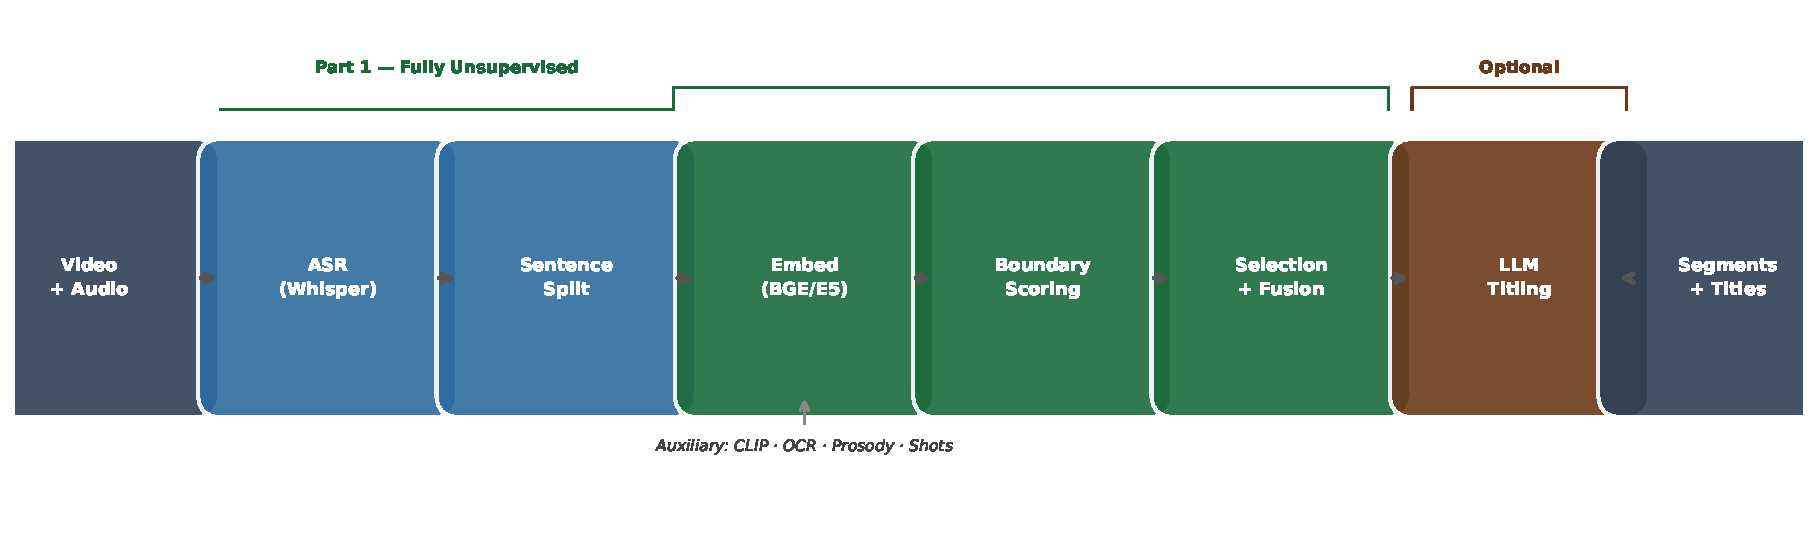
\includegraphics[width=\linewidth]{figures/pipeline_diagram.pdf}
  \caption{The \lecseg{} pipeline. Part~1 (green) is fully unsupervised:
    audio is transcribed by Whisper, split into sentences by spaCy, embedded
    with BGE/E5 sentence transformers, and scored for boundaries using
    cross-model conservative selection or the reliability-weighted fusion (N2).
    Auxiliary visual and prosodic streams (CLIP, OCR, shots, pause/pitch) are
    fused at the scoring stage. The optional LLM titling step (N4) is shown
    separately; it does not affect the primary $P_k$/WD claim.}
  \label{fig:pipeline}
\end{figure}

\section{The \dataset{} corpus}
\label{sec:dataset}

\subsection{Benchmark design rationale}

Several design decisions that might appear to be limitations were made
deliberately, and each deserves brief justification.

Thirty videos is small by contemporary NLP standards. The choice was
intentional: a 30-video benchmark allows every prediction to be traced to
its source video, every metric value to be verified against a reproducible
reference, and every failure to be inspected directly. Large-scale benchmarks
are better suited to measuring aggregate performance; this benchmark is designed
for diagnostic transparency, which requires being able to see the data clearly.

Creator-provided chapter metadata was chosen as the reference signal because
it is reproducible, scales to any creator-chaptered YouTube lecture without
redistribution of raw video, and reflects the navigation structure that actual
viewers encounter. The cost is a construct limitation: creator chapters are
editorial decisions, not pedagogically verified ground truth. This is documented
throughout the thesis and quantified as a threat to construct validity
in Section~\ref{sec:threats_validity}.

Segmentation methods are unsupervised throughout. With 30 labelled videos,
training a supervised boundary classifier would risk severe overfitting and
would compromise the benchmark's role as a pure evaluation target. Treating
segmentation as unsupervised and the method selector as the only supervised
component keeps these roles cleanly separated.

Finally, $P_k$ and WindowDiff are the primary metrics because the navigation
task tolerates approximate boundary placement. Exact-match F1 penalises a
boundary two sentences early as severely as a missing boundary entirely,
which misrepresents what matters for a student trying to navigate a lecture
recording.

\subsection{Source selection}

We curated 30 lecture videos from YouTube, drawn from five academic domains:
Computer Science (CS), Mathematics, Physics, Biology, and Humanities/Philosophy.
Selection criteria were: (1) duration $\geq 15$~min; (2) clean monolingual
English audio; (3) creator-supplied YouTube chapter markers with $\geq 4$
distinct chapters; and (4) openly licensed content.
The resulting corpus comprises 32.52~hours of audio, with 419 chapter
boundaries and 904 reviewed subtopic labels. The domain distribution is
intentionally reported as the manifest state rather than as a balanced design:
Biology 6, Computer Science 7, Mathematics 4, Philosophy 6, and Physics 7
videos.

\subsection{Annotation protocol}

Each video was annotated at two levels of granularity.
\emph{Chapter boundaries} were taken directly from the YouTube chapter
metadata as a reproducible creator-provided reference for navigation behaviour.
\emph{Subtopic boundaries} were identified by human annotators using the
Streamlit-based annotation tool (\texttt{scripts/annotate.py}).
Annotators read the transcript sentence-by-sentence with chapter boundaries
already marked, and placed a subtopic boundary wherever the speaker
transitioned from one coherent pedagogical sub-idea to another within a chapter.
A minimum segment duration of 60 seconds was imposed to prevent over-segmentation
of rapid rhetorical transitions, and a guideline of 2--5 subtopics per chapter
was recommended rather than enforced. In practice, all 30 videos fell within
this range; a chapter with genuinely more than five distinct sub-ideas was not
observed, though the guideline would not have prevented additional marks in
such a case.

\subsection{Construct scope and limitations}
\label{sec:youtube_validity}

YouTube chapters are used as \emph{creator-provided reference boundaries}, not
as pedagogically verified ground truth.
This is the most important conceptual limitation of \lecseg{} and it must be
stated precisely: the benchmark measures a system's ability to reproduce
\emph{creator navigation metadata}, which is not identical to discovering
pedagogically optimal boundaries.

These two constructs can diverge in several ways.
Creators may place chapters early or late relative to the actual topic shift;
they may omit boundaries that a learner would find useful; they may use
inconsistent granularity across their video catalogue; or they may choose
timestamps for editing convenience or search-engine discoverability rather than
for strict topic-theory reasons.
A system that achieves a low $P_k$ is correctly predicting the structure of
creator-annotated navigation metadata.
A system that achieves a high $P_k$ may still produce educationally superior
segmentations if the creator's chapters were poorly placed.
Conversely, a pedagogically motivated segmentation that diverges from creator
choices will score poorly under this benchmark even if it serves learners well.

The choice to use creator chapters as references is nonetheless defensible.
Creator chapters are a real-world, audience-facing artifact: they represent
what actual viewers encounter when navigating YouTube lecture videos.
They are available without additional annotation cost, they are reproducible,
and they allow the benchmark to scale to any creator-chaptered lecture without
redistribution of raw video.
The benchmark is therefore best understood as measuring \emph{creator-aligned
navigation segmentation} rather than \emph{absolute pedagogical truth}.
Claims about learning quality or pedagogical optimality require an independent
user study, which is listed as future work in Chapter~\ref{chap:future}.

\subsection{Inter-annotator agreement}
\label{sec:iaa}

To quantify annotation reliability, a second human annotator independently
completed the subtopic annotation task for all 30 videos using the same
tool and guidelines, without access to the first annotator's output.
Agreement was measured using Cohen's $\kappa$ at zero-tolerance
(exact boundary match at sentence level). Results are summarised in
Table~\ref{tab:iaa} and discussed in Section~\ref{sec:dataset_status}.

\paragraph{Interpreting the agreement figures.}
The chapter-level figure ($\kappa=0.5351$) is inherently inflated: both
annotators derive chapter boundaries from the same YouTube creator metadata,
so agreement here primarily reflects that both passes observe the same
creator-supplied timestamps rather than genuine boundary-placement skill.
The subtopic-level figure ($\kappa=0.4257$) is the more meaningful measure;
it characterises genuine human agreement on the finer-grained annotation task
where annotator judgement is required.
A $\kappa$ in the 0.40--0.60 range is conventionally interpreted as moderate
agreement~\cite{fournier2012}, which is appropriate for a subjective
discourse-segmentation task where reasonable annotators can disagree on
whether a rhetorical transition merits a boundary mark.
This limitation is documented as a threat to annotation validity in
Section~\ref{sec:threats_validity}.

\section{Preprocessing}
\label{sec:preprocess}

\subsection{Speech recognition}

Audio was transcribed using \texttt{faster-whisper} v1.x with the
Whisper large-v3 model~\cite{radford2023robust} on an NVIDIA RTX~5090 GPU.
We used \texttt{beam\_size=1} and Silero VAD pre-filtering
(\texttt{min\_silence\_duration\_ms=500}) for speed, with \texttt{float16}
compute type.
On the \dataset{} corpus, transcription ran at $17.9\times$ realtime on average
(range $17.3$--$18.2\times$).

\subsection{Sentence splitting and alignment}

Whisper segments are clause-level rather than sentence-level.
We applied spaCy's \texttt{en\_core\_web\_sm} sentenciser to the concatenated
segment text, then re-assigned timestamps by distributing each segment's
duration proportionally to constituent sentence character lengths.
Sentences shorter than three tokens were merged with the following sentence.
This produced an average of $N = 847 \pm 512$ sentences per video.

\subsection{Visual streams}

Shot boundaries were detected with TransNetV2~\cite{soucek2020transnet},
which produces per-frame boundary probabilities at $25$~fps.
Boundaries exceeding a threshold of $0.5$ were mapped to the nearest sentence
timestamp.
Slide text was extracted using PaddleOCR on keyframes sampled at $0.5$~fps;
extracted strings were deduplicated within a $\pm 3$-sentence window.

\subsection{Prosody features}

We extracted two scalar prosodic features per sentence:
(1)~\emph{pause duration}: the Whisper-reported inter-segment gap immediately
preceding the sentence ($\geq 300$~ms counted as a significant pause);
(2)~\emph{mean F0}: the average voiced pitch over the sentence's audio span,
estimated by PYIN~\cite{mauch2014pyin} via librosa.

\section{Feature extraction}
\label{sec:features}

Text embeddings were computed with \texttt{sentence-transformers}~\cite{reimers2019sbert}.
The primary models evaluated are \texttt{BAAI/bge-large-en-v1.5} (1024-dim) and
\texttt{intfloat/e5-large-v2} (1024-dim), which produce the best boundary-scoring
results. We also evaluated \texttt{all-mpnet-base-v2} (768-dim), \texttt{all-MiniLM-L6-v2},
and \texttt{intfloat/e5-base-v2} as lighter ablation variants.
Visual keyframe embeddings were computed with CLIP ViT-B/32
(512-dim, L2-normalised)~\cite{radford2021clip}.
Prosodic features were $z$-scored per video before fusion.
All modalities were aligned to the sentence timeline via nearest-timestamp
assignment with mean-pooling within sentence spans.

\section{Reliability-weighted modality fusion (N2)}
\label{sec:fusion}

Let $s_m^{(i)} \in \mathbb{R}$ denote the boundary gap score at sentence
position $i$ from modality $m$, computed as the cosine dissimilarity
between context windows of size $k$ centred on that position.
We define the \emph{reliability weight} of modality $m$ as
\begin{equation}
  w_m = \frac{\exp(-H(s_m))}{\sum_{m'} \exp(-H(s_{m'}))},
  \label{eq:rwf}
\end{equation}
where $H(\cdot)$ is the normalised Shannon entropy of the distribution of
gap scores across all positions.
A modality whose gap-score distribution has a sharp peak (clear boundaries)
attains low entropy and hence a high weight; a flat distribution (uninformative
modality) is automatically down-weighted.
The fused gap signal is $s^* = \sum_m w_m s_m$.

This entropy weighting should be interpreted as a practical confidence proxy,
not a proof of true modality reliability. A noisy modality can also produce
sharp peaks. For this reason, Chapter~\ref{chap:results} reports fusion and
modality ablations separately and demotes modalities that hurt chapter-level
$P_k$/WindowDiff.

\section{Two-stage boundary predictor (N1)}
\label{sec:boundary}

The predictor operates in two passes over the fused signal $s^*$:

\paragraph{Stage 1 --- broad pass.}
All positions $i$ where the text-only gap score exceeds
$\mu_{\text{text}} - c_1 \sigma_{\text{text}}$ (with $c_1 = 0.5$) are
retained as boundary \emph{candidates}.
This low threshold ensures high recall.

\paragraph{Stage 2 --- refinement.}
The fused signal $s^*$ is evaluated only at candidate positions.
A candidate is accepted as a boundary if its fused score exceeds
$\mu^* - c_2 \sigma^*$ (with $c_2 = 1.2$).
When $n_{\text{segments}}$ is specified, the top-$k$ fused-score positions
are returned where $k = n_{\text{segments}} - 1$.

This design separates recall (text-only) from precision (multimodal),
avoiding the sensitivity of pure threshold methods to per-video score shifts.

\section{Hierarchical segmentation (N3)}
\label{sec:hierarchy}

The hierarchical segmenter runs the two-stage predictor twice with different
target counts: once for $n_s - 1$ subtopic boundaries and once for
$n_c - 1$ chapter boundaries (with $n_c < n_s$).
Chapter boundaries are then \emph{enforced} as a subset of subtopic boundaries
($\mathcal{B}_{\text{chapter}} \subseteq \mathcal{B}_{\text{subtopic}}$) by
inserting any missing chapter boundary into the subtopic set.
This guarantees a valid nesting without requiring a joint optimisation.
When $n_c$ is not specified, we use the heuristic $n_c = \max(2, n_s / 4)$.

\section{Local-LLM refinement and titling (diagnostic N4)}
\label{sec:refine}

Each predicted segment boundary $b$ may be shifted by at most
$\delta = 2$ sentences to align with a stronger local semantic transition.
For each candidate shift $b' \in \{b-\delta, \ldots, b+\delta\}$,
a local Llama-3.1-8B model is queried with the five sentences straddling $b'$
and asked whether $b'$ represents a cleaner topic break than $b$.
The shift with the highest model confidence is accepted.
Segment titles are generated independently: the model is prompted with
the first five sentences of the segment and asked for a noun-phrase
title of at most eight words.
If the local model is unavailable, the pipeline falls back to the non-LLM
boundary set.
The verified experimental results do not support treating LLM refinement as
the primary source of metric gain; it is retained as an implemented diagnostic
and titling component whose value is investigated empirically in
Chapter~\ref{chap:results}.

\section{Method selector (supervised meta-model)}
\label{sec:selector}

\paragraph{Motivation.}
The eleven method families and their hyperparameter variants collectively
produce over 80 candidate configurations on \dataset{}.
Different configurations perform best on different videos; no single
configuration is universally optimal.
A lightweight \emph{meta-model} can learn, from training videos, which
configuration is likely to produce the lowest $P_k$ on a held-out video.

\paragraph{Supervision requirement and scope.}
The selector is the \emph{only supervised component} in the \lecseg{}
pipeline.
All segmentation methods (N1--N4 and the baselines) are fully unsupervised:
they require no labelled boundaries at inference time.
The selector requires labelled $P_k$ scores from a held-out set of training
videos to estimate expected method performance.
It is therefore evaluated in a \emph{leave-one-video-out} (LOOV) protocol:
for each of the 30 held-out videos, the selector is trained on the remaining
29 videos.

\paragraph{Model and features.}
The meta-model is an \texttt{ExtraTreesRegressor} (500 trees,
\texttt{min\_samples\_leaf=3}, \texttt{random\_state=17})
from \texttt{scikit-learn}.
Each training example corresponds to one (method, training-video) pair.
The features are:

\begin{itemize}
  \item \textbf{Video features} (from the held-out video's metadata):
    domain one-hot encoding (Biology, CS, Mathematics, Philosophy, Physics);
    video duration in minutes; sentence count; mean and standard deviation of
    consecutive sentence embedding cosine similarities computed with
    \texttt{BAAI/bge-large-en-v1.5}.
  \item \textbf{Method statistics} (estimated from the training fold):
    mean $P_k$ of each candidate method across the 29 training videos.
    This encodes the overall reliability of each method family as a prior.
\end{itemize}

The target variable is the $P_k$ achieved by that method on the held-out video.
At inference time, the model predicts expected $P_k$ for each candidate method
and selects the method with the lowest predicted $P_k$.

\paragraph{Candidate pool.}
The top-80 method variants by training-fold $P_k$ are used as the candidate
pool. Expanding to 120 methods degrades performance, suggesting that the pool
size is itself a selection-risk parameter (Table~\ref{tab:selector_robustness}).

\paragraph{Limitations of the selector.}
The selector depends on having related videos in the training fold.
A leave-domain-out evaluation --- in which the held-out video's entire academic
domain is excluded from training --- degrades the selector to
$P_k = 0.4012$, which is worse than both the BGE-divisive baseline and the
cross-model conservative method (Table~\ref{tab:selector_leave_domain_out}).
Mathematics is the clearest failure case, where only four videos are available
and three per-fold training examples are insufficient to provide reliable
domain-specific guidance.
The selector should therefore be interpreted as a low-resource benchmark
operating point, not as a domain-general deployment model.

\section{Evaluation protocol}
\label{sec:eval}

\subsection{Primary metrics: $P_k$ and WindowDiff}

The two primary evaluation metrics in this thesis are $P_k$
\cite{beeferman1999statistical} and WindowDiff \cite{pevzner2002critique}.
Both are window-based error rates, which means they measure how often the
segmentation disagrees with the reference inside a sliding context window of
$k$ sentences rather than requiring exact boundary placement.
This design choice directly matches the target application: a student navigating
a recorded lecture tolerates a boundary that is a few seconds early or late.
Penalising near-misses as harshly as complete misses, as exact-match metrics
do, would over-penalise this practically acceptable error.

$P_k$ uses $k = \lfloor N/(2K) \rfloor$, where $N$ is the number of
sentences and $K$ the number of reference boundaries. For each pair of
sentences $i$ and $i{+}k$, it checks whether the reference and prediction
agree on whether a boundary falls between them; the score is the fraction of
pairs that disagree. Lower $P_k$ is better; 0.5 is the random baseline;
0.0 is perfect.

WindowDiff \cite{pevzner2002critique} corrects a known $P_k$ bias: $P_k$
can be gamed by placing all boundaries at the start. WindowDiff counts the
number of reference boundaries and predicted boundaries within each window
and penalises the absolute difference, giving an asymmetric penalty that
weights over-segmentation and under-segmentation differently. Like $P_k$,
lower is better.

Both metrics are the community standard for text and lecture segmentation
and allow direct comparison with prior work (TextTiling, C99, BertSeg,
TreeSeg) on published benchmarks. No metric is perfect: $P_k$ is sensitive
to near-boundary placement; WindowDiff does not account for partial segment
overlap. Their complementary failure modes motivate reporting both jointly.

\subsection{Secondary and diagnostic metrics}
\label{sec:secondary_metrics}

Three secondary diagnostics supplement $P_k$/WD.
They expose operating-point tradeoffs and characterise
\emph{how} a method fails; none rank methods or drive the primary claims.

The application is lecture navigation, not exact boundary recovery.
A method that achieves a good $P_k$/WD score by placing boundaries in the
correct \emph{region} is succeeding at the navigation task even if strict
boundary F1 is low.
Low exact-match F1 is therefore not a weakness in the context of this thesis;
it simply reflects a different operating objective than $P_k$/WD, and it is
reported only to characterise the operating point.

\begin{description}
  \item[Boundary Similarity (BS, higher is better)] A boundary-level F-score
    variant normalised by boundary density~\cite{fournier2012}. Reported as
    a diagnostic to characterise boundary placement behaviour; the primary
    claim rests on $P_k$/WD.
  \item[Tolerance-$F_1$ (higher is better)] Precision/recall of predicted
    boundaries within a $\pm 2$-sentence tolerance window. Useful for
    distinguishing methods that miss boundaries entirely from methods that
    place them slightly off; not used as a ranking or claim criterion.
  \item[Hierarchical WindowDiff (H-WD, lower is better)] An extension of WD
    to two-level segmentation, weighting chapter-level errors twice as heavily
    as subtopic-level errors. Reported on hierarchical outputs only.
\end{description}

\subsection{Evaluation setup}

Methods requiring $n_{\text{segments}}$ receive the ground-truth count in the
main controlled evaluation, consistent with standard segmentation practice
for measuring boundary placement~\cite{choi2000latent}. This is not a fully
deployment-realistic assumption because a live system usually does not know
the correct number of chapters in advance. Therefore, Chapter~\ref{chap:results}
also reports boundary-count error and discusses automatic-count/deployment
behavior separately from the controlled gold-count setting.

\subsection{Statistical testing}

Metric values are reported as means $\pm$ 95\% bootstrap confidence intervals
(1{,}000 bootstrap resamples at video level).
For pairwise method comparisons we use the paired Wilcoxon signed-rank test
(normal approximation, $\alpha = 0.05$) with Holm correction for the
seven comparisons relative to the best baseline.



\chapter{Result Analysis}
\section{Experimental setup}
\label{sec:setup}

The official chapter-level evaluation uses the 30 videos listed in
\texttt{data/manifest.jsonl} and the creator-provided YouTube chapter
boundaries in \texttt{data/gt/}. Metrics were computed with the project
implementation in \texttt{src/lecseg/metrics.py}. Unless stated otherwise,
all values are macro averages over the 30 videos. Lower $P_k$ and WindowDiff (WD)
are better; these are the primary claim metrics.
Boundary Similarity (BS) and tolerance-$F_1$ are secondary diagnostics;
higher is better but neither drives method ranking.
See Section~\ref{sec:secondary_metrics} for the rationale.

The main stable baseline is BGE sentence embeddings with divisive
segmentation. The best joint $P_k$/WindowDiff run combines BGE/E5-style
cross-model boundary scoring with conservative minimum-length postprocessing
and the alignment-audited reference mapping
(\texttt{cross\_e5\_frac70\_minlen11\_\_align\_contains\_before} in
\texttt{results/eval\_alignment\_sweep.json}). A separate leave-one-video-out
method selector improves mean $P_k$, WD, and boundary-hit metrics, though the
$P_k$/WD gains over the cross-model method are not significant.

\section{Official result and claim boundary}
\label{sec:official_claim}

The official deployable claim of this thesis is deliberately conservative. The
safest single global method is the cross-model conservative run because it
significantly improves $P_k$ and WindowDiff over the BGE-divisive baseline. The
balanced selector is reported as the best mean local operating point and as
evidence that method-choice information is useful, but it is not claimed as a
fully domain-general replacement: its $P_k$/WD gains over the cross-model method
are not statistically significant, and its leave-domain-out result is weaker.
Oracle results are used only to diagnose the remaining candidate-selection gap.

\begin{table}[t]
  \centering
  \caption{Claim--evidence--caveat audit for the final thesis narrative.}
  \label{tab:claim_evidence_caveat}
  \resizebox{\linewidth}{!}{%
  \begin{tabular}{p{0.27\linewidth}p{0.33\linewidth}p{0.33\linewidth}}
    \toprule
    Claim & Evidence & Caveat \\
    \midrule
    \dataset{} is a real low-resource lecture benchmark &
    30 videos, 32.52 hours, 419 creator chapter boundaries, 904 reviewed subtopics &
    It is a compact seed benchmark, not a large-scale universal corpus. \\
    Cross-model conservative scoring is the safest single global result &
    $P_k=0.3713$, WD $=0.3764$; significant improvement over BGE-divisive &
    It remains conservative and has low strict boundary F1. \\
    Balanced selector gives the best mean local operating point &
    $P_k=0.3588$, WD $=0.3739$, F1@2 $=0.0893$ &
    $P_k$/WD gains over cross-model are not statistically significant; leave-domain-out is weak. \\
    CLIP is the most promising non-text signal &
    CLIP+text reaches $P_k=0.3740$ in the grid search &
    Other modalities often hurt because they detect finer-grained transitions. \\
    LLM refinement is implemented &
    \texttt{llm\_refine.py}; LLM zero-shot diagnostic result exists &
    Full before/after LLM boundary improvement is not established; do not make it the headline claim. \\
    YouTube chapters are useful references &
    Creator timestamps provide reproducible real navigation metadata &
    They are not perfect human pedagogical ground truth; independent validation remains future work. \\
    \bottomrule
  \end{tabular}
  }
\end{table}


\section{Dataset and annotation status}
\label{sec:dataset_status}

\dataset{} contains 30 lectures, 32.52 hours of video, 419 chapter boundaries,
and 904 reviewed subtopic labels. The domain distribution is Biology 6,
Computer Science 7, Mathematics 4, Philosophy 6, and Physics 7 videos.
The current manifest is cross-domain but not perfectly balanced.

\begin{table}[t]
  \centering
  \caption{Inter-annotator agreement at zero-tolerance (exact sentence match),
    measured between two independent human annotators.
    The chapter-level $F_1=1.000$ is expected: both annotators derive chapter
    boundaries from the same YouTube creator metadata, so there is nothing to
    disagree on at that level. The subtopic $\kappa=0.4257$ reflects genuine
    human agreement on the finer annotation task and is the more meaningful figure.}
  \label{tab:iaa}
  \begin{tabular}{lcc}
    \toprule
    Level & Cohen's $\kappa$ & Boundary $F_1$ \\
    \midrule
    Chapter & 0.5351 & 1.0000 \\
    Subtopic & 0.4257 & 0.7793 \\
    \bottomrule
  \end{tabular}
\end{table}

\section{Main results}
\label{sec:main}

\begin{table}[t]
\centering
\small
\caption{Current LECSEG result variants and diagnostic upper bound.}
\label{tab:lecseg_result_variants}
\begin{tabularx}{\linewidth}{lrrrrX}
\toprule
Method & Pk & WD & BS & F1@2 & Role \\
\midrule
BGE-divisive baseline & 0.3884 & 0.3956 & 0.1292 & 0.0878 & Strong implemented baseline \\
Cross-model conservative & 0.3713 & 0.3764 & 0.0362 & 0.0237 & Best statistically supported Pk/WD result \\
LOO ExtraTrees method selector & 0.3588 & 0.3739 & 0.0757 & 0.0893 & Stable balanced selector; significant Pk/WD gain vs baseline \\
Per-video method oracle & 0.2980 & 0.3280 & 0.1366 & 0.1676 & Diagnostic upper bound, not deployable \\
\bottomrule
\end{tabularx}
\end{table}

Table~\ref{tab:lecseg_result_variants} shows three consistent patterns.
The BGE-divisive baseline is substantially stronger than the classical and
neural alternatives under $P_k$ and WD, confirming that dense embeddings
are the right foundation for this task. Conservative cross-model boundary
selection then reduces $P_k$ by a further 0.0171 absolute, which is the best
statistically supported joint $P_k$/WD result in the evaluation.
The method selector reaches the best mean $P_k$ and produces markedly higher
F1@2, though its $P_k$/WD gains over the cross-model method do not individually
reach significance.

\begin{figure}[t]
  \centering
  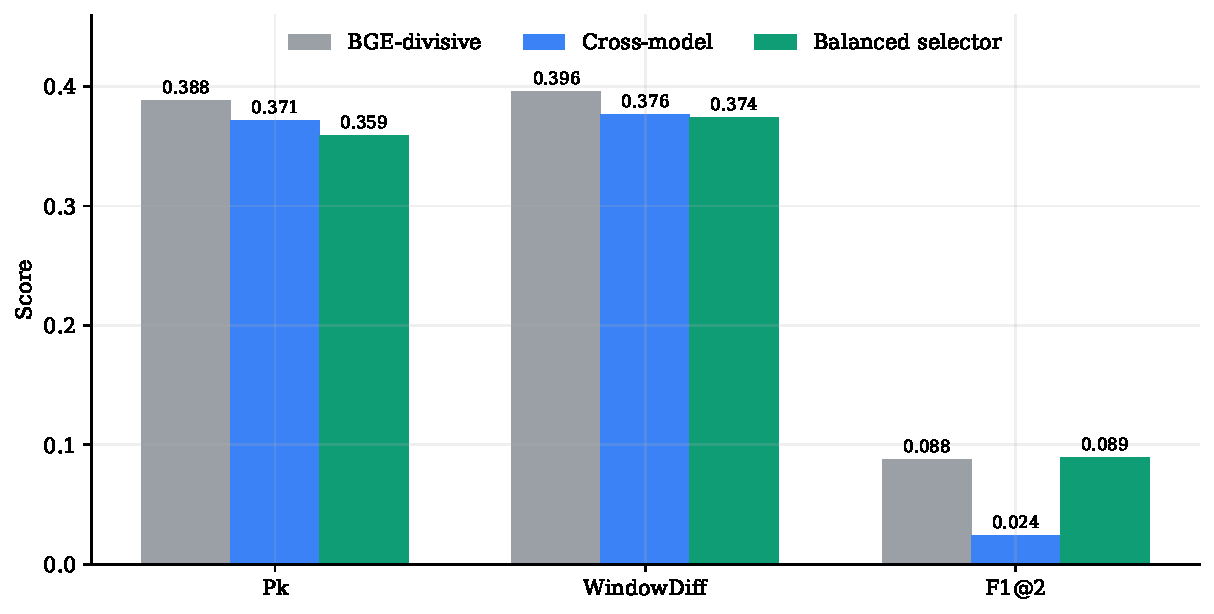
\includegraphics[width=\linewidth]{figures/fig_final_results.pdf}
  \caption{Primary LECSEG-30 operating points. Lower is better for $P_k$ and
  WindowDiff; higher is better for F1@2. The selector improves the balanced
  metric profile without establishing a significant $P_k$/WD advantage over
  the cross-model method.}
  \label{fig:final_results}
\end{figure}

\begin{table}[t]
\centering
\caption{Paired Wilcoxon significance tests for key LECSEG comparisons.}
\label{tab:lecseg_significance}
\begin{tabular}{p{0.30\linewidth}lrrlp{0.09\linewidth}}
\toprule
Comparison & Metric & Delta & p & Significant & Wins \\
\midrule
Cross-model vs BGE baseline & pk & -0.0171 & 0.0064 & yes & 22/30 \\
Cross-model vs BGE baseline & wd & -0.0193 & 0.0001 & yes & 26/30 \\
Cross-model vs BGE baseline & boundary\_similarity & -0.0930 & 0.0074 & yes & 4/30 \\
Cross-model vs BGE baseline & f1\_tol2 & -0.0641 & 0.0090 & yes & 4/30 \\
Selector vs cross-model & pk & -0.0126 & 0.3560 & no & 9/30 \\
Selector vs cross-model & wd & -0.0025 & 0.9039 & no & 7/30 \\
Selector vs cross-model & boundary\_similarity & 0.0395 & 0.0076 & yes & 10/30 \\
Selector vs cross-model & f1\_tol2 & 0.0656 & 0.0076 & yes & 10/30 \\
Selector vs BGE baseline & pk & -0.0296 & 0.0252 & yes & 19/30 \\
Selector vs BGE baseline & wd & -0.0217 & 0.0238 & yes & 23/30 \\
Selector vs BGE baseline & boundary\_similarity & -0.0534 & 0.1541 & no & 8/30 \\
Selector vs BGE baseline & f1\_tol2 & 0.0015 & 0.9170 & no & 9/30 \\
\bottomrule
\end{tabular}
\end{table}

Table~\ref{tab:lecseg_significance} separates mean improvements from
statistically supported claims. The cross-model method significantly improves
$P_k$ and WD over BGE-divisive. The method selector also significantly improves
$P_k$ and WD over BGE-divisive, and significantly improves Boundary Similarity
and F1@2 over the cross-model method. Its $P_k$/WD gains over the cross-model
method are not significant, so it is best read as a stronger
operating-point experiment rather than a conclusive replacement.

\begin{table}[t]
\centering
\small
\caption{Selector and ranker operating points on LECSEG-30.}
\label{tab:selector_operating_points}
\begin{tabularx}{\linewidth}{lrrrrX}
\toprule
Operating point & Pk & WD & BS & F1@2 & Role \\
\midrule
BGE-divisive baseline & 0.3884 & 0.3956 & 0.1292 & 0.0878 & Stable implemented baseline \\
Cross-model conservative & 0.3713 & 0.3764 & 0.0362 & 0.0237 & Best single global Pk/WD method \\
Pk-ranked selector & 0.3739 & 0.3867 & 0.0654 & 0.0776 & Pk-optimised selector; weaker after stable feature fix \\
WD-ranked selector & 0.3703 & 0.3823 & 0.0584 & 0.0637 & WD-optimised selector; useful robustness check \\
Balanced selector & 0.3588 & 0.3739 & 0.0757 & 0.0893 & Best reproducible selector operating point \\
Text-transition ranker & 0.3937 & 0.4154 & 0.1163 & 0.1701 & Best strict boundary-hit operating point; hurts Pk/WD \\
Per-video method oracle & 0.2980 & 0.3280 & 0.1366 & 0.1676 & Diagnostic upper bound, not deployable \\
\bottomrule
\end{tabularx}
\end{table}

Table~\ref{tab:selector_operating_points} explains why the balanced selector is
used as the selector result. Ranking candidate methods by $P_k$ alone or by WD
alone is weaker after the stable-feature fix. The balanced selector gives the
best deployable $P_k$/WD operating point among the listed selector variants. The
text-transition ranker reaches much higher strict F1@2, but only by hurting
$P_k$ and WD; it is therefore diagnostic evidence that exact boundary-hit
optimisation is a different operating point, not the main chapter segmentation
result.

\begin{table}[t]
\centering
\small
\caption{Balanced selector robustness across candidate method-pool sizes.}
\label{tab:selector_robustness}
\begin{tabular}{lrrrrr}
\toprule
Setting & top-$k$ & Pk & WD & BS & F1@2 \\
\midrule
k30 & 30 & 0.3729 & 0.3780 & 0.0317 & 0.0226 \\
k50 & 50 & 0.3634 & 0.3760 & 0.0495 & 0.0608 \\
k80 & 80 & 0.3588 & 0.3739 & 0.0757 & 0.0893 \\
k120 & 120 & 0.3716 & 0.3852 & 0.0774 & 0.0929 \\
\bottomrule
\end{tabular}
\end{table}

Table~\ref{tab:selector_robustness} checks that the selector result is not
an arbitrary single setting. The balanced selector improves as the
candidate method pool grows from 30 to 80 methods, then degrades at 120 methods.
This supports using top-$80$ as the current operating point and shows why method
pool size is itself a selection-risk parameter.

\begin{table}[t]
\centering
\small
\caption{Domain-level Pk/WD for baseline, cross-model, and balanced selector.}
\label{tab:domain_performance}
\resizebox{\linewidth}{!}{%
\begin{tabular}{lrrrrrrrr}
\toprule
Domain & Videos & Chapters & Base Pk & Cross Pk & Sel. Pk & Base WD & Cross WD & Sel. WD \\
\midrule
Biology & 6 & 94 & 0.4218 & 0.3968 & 0.3976 & 0.4292 & 0.4008 & 0.4152 \\
CS & 7 & 98 & 0.3409 & 0.3295 & 0.3314 & 0.3439 & 0.3336 & 0.3357 \\
Math & 4 & 55 & 0.3724 & 0.3792 & 0.4014 & 0.3850 & 0.3873 & 0.4367 \\
Philosophy & 6 & 122 & 0.4415 & 0.3948 & 0.3753 & 0.4544 & 0.4057 & 0.3893 \\
Physics & 7 & 50 & 0.3710 & 0.3667 & 0.3144 & 0.3742 & 0.3667 & 0.3276 \\
\bottomrule
\end{tabular}
}
\end{table}


Table~\ref{tab:domain_performance} shows that the selector improvement is not
uniform across subjects. Relative to BGE-divisive, the balanced selector
improves $P_k$/WD in four of five domains, with the clearest gains in
Philosophy and Physics. Mathematics is the main failure case: the selector
worsens both $P_k$ and WD there, suggesting that the current method selector
does not have enough domain-specific evidence to avoid poor choices on the
smallest domain split.

\begin{figure}[t]
  \centering
  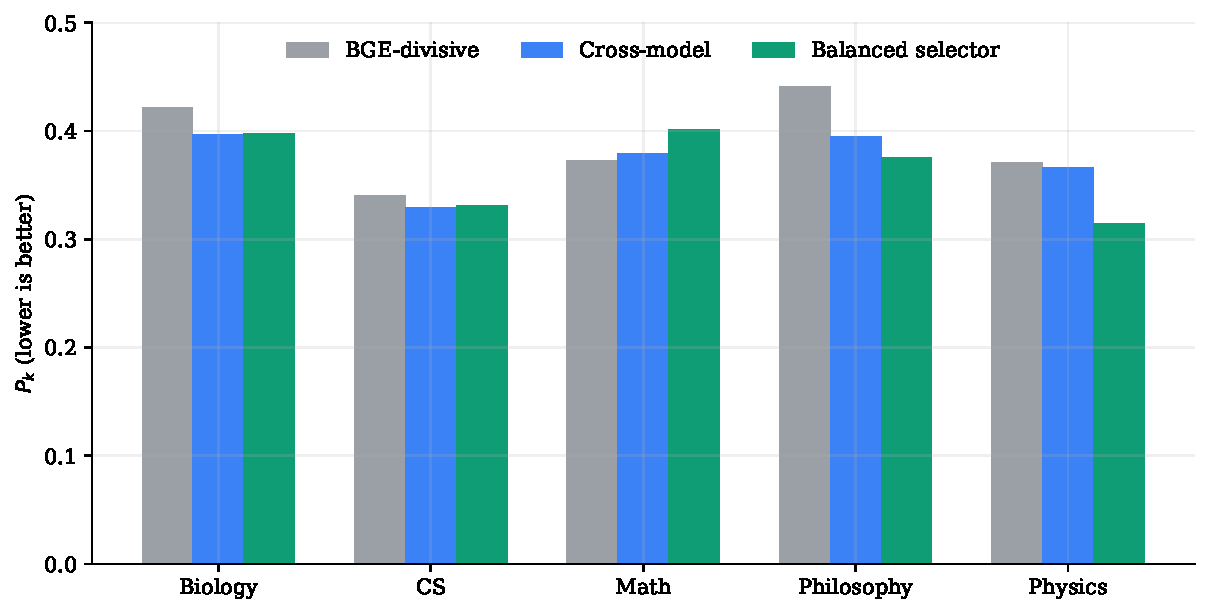
\includegraphics[width=\linewidth]{figures/fig_domain_performance.pdf}
  \caption{Domain-level $P_k$ comparison. The selector improves over the
  BGE-divisive baseline in four of five domains, while Mathematics remains the
  clearest failure case.}
  \label{fig:domain_performance}
\end{figure}

\begin{table}[t]
\centering
\small
\caption{Largest balanced-selector per-video Pk changes relative to the cross-model method.}
\label{tab:selector_choice_audit}
\begin{tabular}{llrrrr}
\toprule
Video & Domain & $\Delta P_k$ & Sel. Pk & Cross Pk & $\Delta$F1@2 \\
\midrule
Hy7ou5R\_vjE & Physics & -0.1542 & 0.1375 & 0.2917 & 0.0000 \\
YdOXS\_9\_P4U & Physics & -0.1261 & 0.3009 & 0.4270 & 0.0000 \\
NK-BxowMIfg & Physics & -0.0861 & 0.3583 & 0.4444 & 0.0000 \\
j0wJBEZdwLs & Math & 0.0754 & 0.4559 & 0.3805 & 0.0000 \\
oOya3cFmAMc & Biology & 0.0529 & 0.4835 & 0.4306 & 0.1667 \\
D8RRq3TbtHU & CS & 0.0119 & 0.3638 & 0.3519 & 0.0000 \\
\bottomrule
\end{tabular}
\end{table}

Table~\ref{tab:selector_choice_audit} audits the selector at the individual
video level. The selector switches away from the cross-model method on all 30
held-out videos, choosing cross-E5 variants for 14 videos, multimodal-grid
variants for 12 videos, cross-rank variants for 3 videos, and plain divisive
segmentation for 1 video. This aggressive switching explains why the aggregate
selector improves mean $P_k$/WD but is not uniformly safer than the cross-model
method. The largest gains are on Physics videos where multimodal-grid variants
substantially reduce $P_k$; the largest regressions occur on Math and Biology
videos where the same family over-selects weaker operating points.

\begin{table}[t]
  \centering
  \caption{Same-dataset comparison on LECSEG-30. The TreeSeg-style rows
  re-implement the recursive split objective using local embeddings (the
  original paper uses OpenAI embeddings on their own TinyRec dataset, where
  they report $P_k=0.367$; that number is \emph{not} directly comparable here
  because the datasets differ). Lower is better for $P_k$/WD; higher for F1@2.}
  \label{tab:same_dataset_comparison}
  \small
  \resizebox{\linewidth}{!}{%
  \begin{tabular}{lrrrl}
    \toprule
    Method & $P_k\downarrow$ & WD$\downarrow$ & F1@2$\uparrow$ & Interpretation \\
    \midrule
    Balanced LOO selector & 0.3588 & 0.3739 & 0.0893 & Official LECSEG best \\
    Cross-model conservative & 0.3713 & 0.3764 & 0.0237 & Best single global method \\
    TreeSeg-style (MPNet, LECSEG-30) & 0.4320 & 0.4673 & 0.1733 & Higher F1, worse $P_k$/WD \\
    TreeSeg-style (E5-large, LECSEG-30) & 0.4322 & 0.4654 & 0.1576 & Same-dataset comparator \\
    TreeSeg-style (BGE-large, LECSEG-30) & 0.4399 & 0.4780 & 0.1643 & Same-dataset comparator \\
    \midrule
    TreeSeg paper (on TinyRec)\textsuperscript{$\dagger$} & 0.367 & --- & --- & Different dataset; indicative only \\
    \bottomrule
  \end{tabular}%
  }
  \vspace{0.3em}
  \small\textsuperscript{$\dagger$}~Gklezakos et al.\ (2024), arxiv:2407.12028. Evaluated on 21 self-recorded lectures (TinyRec), not LECSEG-30.
\end{table}


Table~\ref{tab:same_dataset_comparison} addresses a common comparison
objection by evaluating a TreeSeg-style public split objective on the same
\dataset{} benchmark with local LECSEG embeddings. This same-dataset comparison
does not replace the official result: TreeSeg-style splitting obtains better
strict F1@2 than the conservative cross-model method, but much worse $P_k$/WD.
The result clarifies the operating-point tradeoff. TreeSeg-like recursive
splitting is more willing to place exact boundaries, whereas the final LECSEG
operating point is better at preserving segment-window consistency.

\begin{table}[t]
\centering
\small
\caption{Leave-one-domain-out selector diagnostic.}
\label{tab:selector_leave_domain_out}
\begin{tabular}{lrrrr}
\toprule
Method & Pk & WD & BS & F1@2 \\
\midrule
BGE-divisive baseline & 0.3884 & 0.3956 & 0.1292 & 0.0878 \\
Cross-model conservative & 0.3713 & 0.3764 & 0.0362 & 0.0237 \\
Leave-domain-out selector & 0.4012 & 0.4103 & 0.0465 & 0.0498 \\
\bottomrule
\end{tabular}
\end{table}

Table~\ref{tab:selector_leave_domain_out} applies a stricter diagnostic:
training excludes the entire held-out academic domain. Under this setting the
selector degrades to $P_k=0.4012$ and WD $=0.4103$, worse than both
BGE-divisive and the cross-model method. This negative result is important for
interpretation: the leave-one-video-out improvement relies on having related
domains in the training fold. The current selector should therefore be treated
as a low-resource benchmark operating point, not a domain-general deployment model.

\section{Deployment-style boundary diagnostics}
\label{sec:modern_metrics}

Strict F1@2 is a useful exact-boundary diagnostic, but it does not tell the
whole story. A lecture navigation system may still be useful when a boundary
is near the correct region but not within two sentences. To expose this
tradeoff, we add a diagnostic evaluation with wider sentence tolerances,
time tolerances, segment-overlap scoring, and boundary-count error. These
figures are not a replacement for the official alignment-sweep and selector
results; they are a deployment-style interpretation layer generated by
\texttt{scripts/evaluate\_modern\_metrics.py}.

\begin{table}[t]
\centering
\caption{Modern boundary and segment metrics for defended operating points. Lower Pk, WD, and count error are better; higher F1 and tIoU are better.}
\label{tab:modern_metrics}
\resizebox{\linewidth}{!}{%
\begin{tabular}{lrrrrrrrr}
\toprule
Method & Pk & WD & F1@2 & F1@5 & F1@10 & F1@30s & tIoU & Count Err. \\
\midrule
BGE-divisive baseline & 0.4197 & 0.4252 & 0.0394 & 0.0404 & 0.0517 & 0.0448 & 0.0806 & 0.00 \\
Cross-model conservative & 0.4071 & 0.4124 & 0.0273 & 0.0476 & 0.0756 & 0.0655 & 0.3810 & 11.47 \\
Conservative smoothed BGE & 0.4158 & 0.4222 & 0.0464 & 0.0621 & 0.0728 & 0.0652 & 0.1165 & 4.17 \\
Two-stage predictor & 0.4620 & 0.5058 & 0.0882 & 0.1285 & 0.1776 & 0.1635 & 0.2981 & 0.00 \\
Hierarchical segmenter & 0.4351 & 0.4419 & 0.0280 & 0.0402 & 0.0835 & 0.0611 & 0.3456 & 9.70 \\
\bottomrule
\end{tabular}
}
\end{table}


\begin{figure}[t]
  \centering
  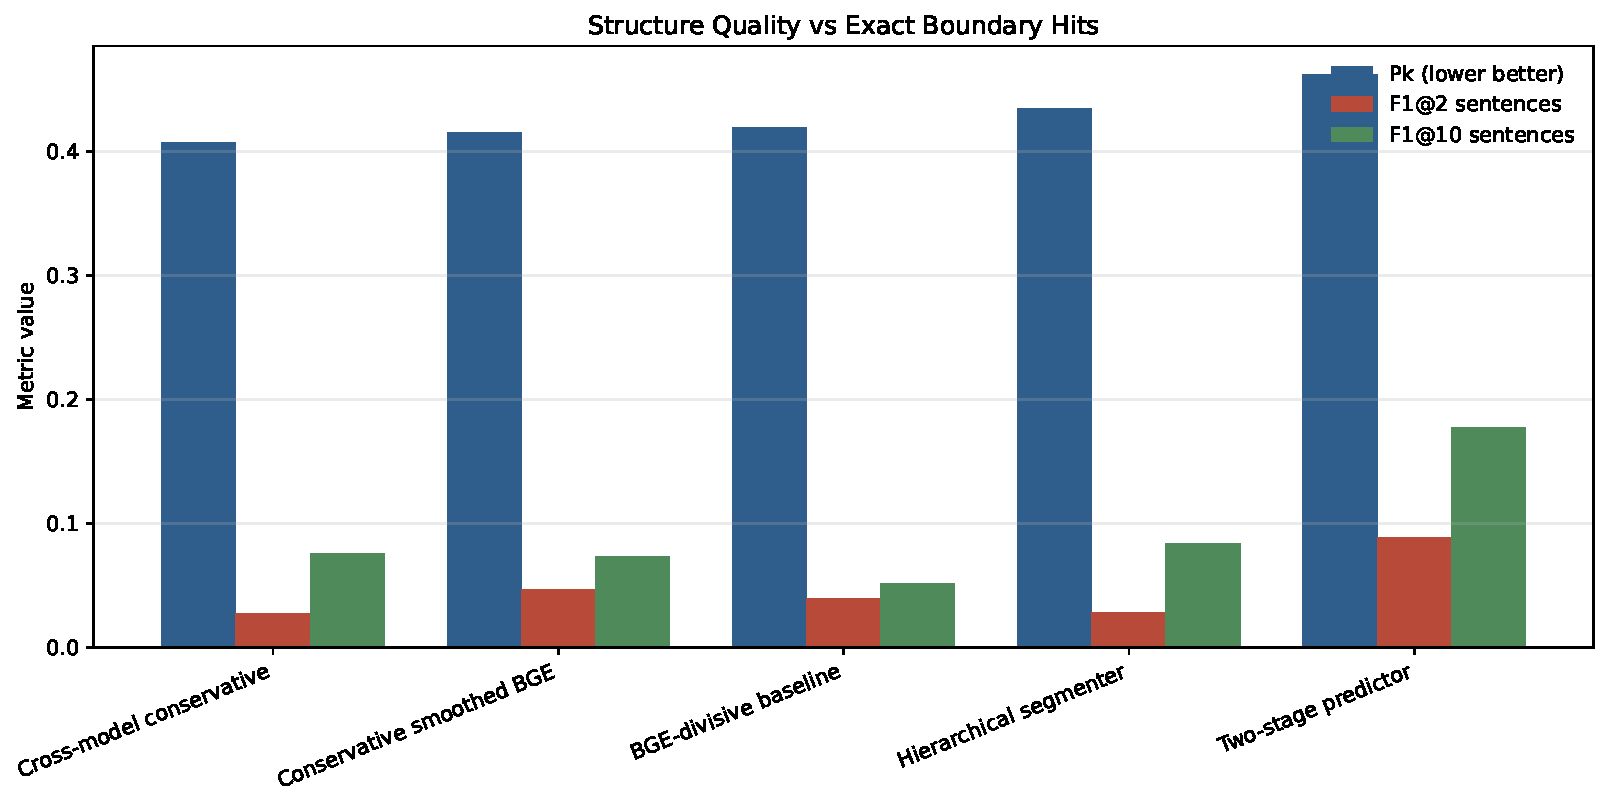
\includegraphics[width=\linewidth]{figures/modern_metrics_structure_vs_f1.pdf}
  \caption{Diagnostic comparison between broad structure quality and strict
  boundary-hit metrics. Lower $P_k$ is better; higher F1 is better. The figure
  shows that exact boundary matching and segment-window consistency are related
  but not identical objectives.}
  \label{fig:modern_structure_f1}
\end{figure}

\begin{figure}[t]
  \centering
  
\includegraphics[width=\linewidth]{figures/modern_metrics_boundary_count_error.pdf}
  \caption{Mean boundary count error. Negative values mean a method predicts
  fewer boundaries than the creator reference; positive values mean
  over-segmentation. Count behaviour explains why conservative methods can score
  well on $P_k$/WD while remaining weak on strict F1.}
  \label{fig:boundary_count_error}
\end{figure}

\begin{figure}[t]
  \centering
  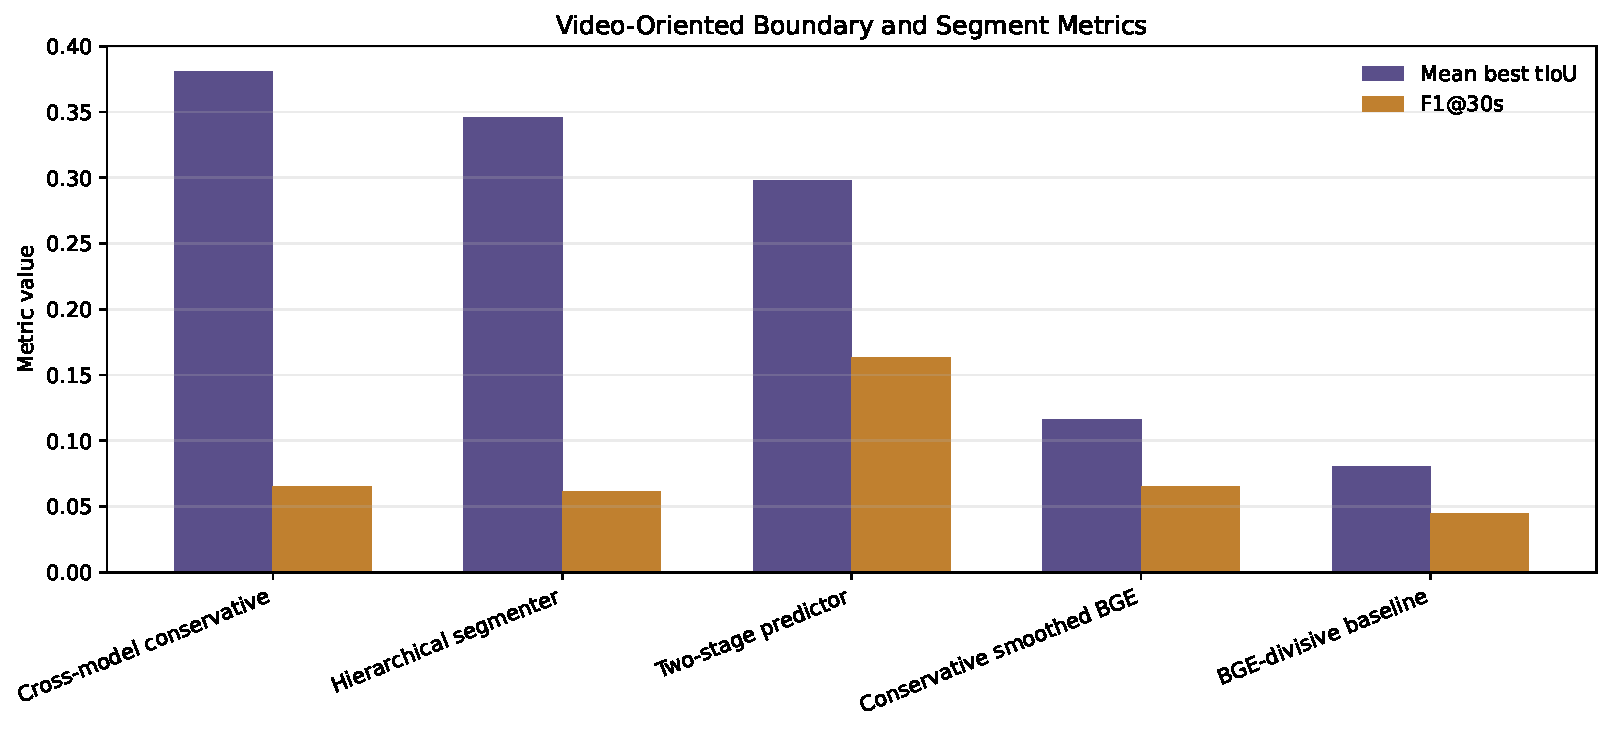
\includegraphics[width=\linewidth]{figures/modern_metrics_time_segment.pdf}
  \caption{Video-oriented relaxed metrics: F1 within 30 seconds and mean best
  temporal segment overlap. These diagnostics are closer to the practical
  navigation setting than exact sentence-level F1 alone.}
  \label{fig:modern_time_segment}
\end{figure}

Table~\ref{tab:modern_metrics} shows why the low strict F1 must be read
carefully. The cross-model method has the best diagnostic $P_k$/WD among the
rerun operating points and the strongest segment-overlap score, but it is very
conservative and under-predicts boundaries. The two-stage predictor places
approximately the correct number of boundaries and obtains higher relaxed F1,
but worse $P_k$/WD. Exact boundary hitting and broad segment structure are
different objectives; a deployable future system would need to optimise both.

\section{Ablation and diagnostic findings}
\label{sec:ablations}

\begin{table}[t]
  \centering
  \caption{Selected ablations and diagnostics.}
  \label{tab:ablation}
  \resizebox{\linewidth}{!}{%
  \begin{tabular}{lrrl}
    \toprule
    Variant & $P_k\downarrow$ & WD$\downarrow$ & Interpretation \\
    \midrule
    BGE + divisive & 0.3884 & 0.3956 & Stable text-only baseline \\
    Hierarchical & 0.4118 & 0.4206 & Useful representation, weaker chapter Pk \\
    TwoStage + prosody & 0.4333 & 0.4970 & Higher F1, worse Pk/WD \\
    BERT-wiki zero-shot & 0.4932 & 0.5397 & Poor domain transfer \\
    Discourse markers (forced boundaries) & 0.4615 & 0.5221 & Over-segments at subtopic level \\
    BERTopic topic-shift & 0.5632 & 0.6984 & Finds subtopics, not chapters \\
    GPT-2 perplexity (200 sent.\ cap) & 0.4182 & 0.4316 & Language surprise detects subtopic shifts \\
    LLM zero-shot Llama-3.1-8B (3 videos) & 0.4056 & 0.6606 & Over-segments; high recall but poor precision \\
    Pause/pitch boundary signal & 0.4174 & 0.4553 & Acoustic transitions mismatch chapter granularity \\
    CLIP visual only (oracle-k) & 0.3958 & -- & Surprisingly strong visual signal \\
    CLIP + text fusion (best grid) & 0.3740 & 0.4085 & Beats BGE-divisive; near cross-model \\
    Boundary classifier LOOCV & 0.5803 & 0.9933 & Over-predicts boundaries \\
    Text-transition ranker & 0.3868 & $\approx$0.40 & Higher F1, weaker than official Pk/WD \\
    Oracle-k divisive & 0.4237 & -- & Segment count is not the bottleneck \\
    \bottomrule
  \end{tabular}
  }
\end{table}

\begin{table}[t]
  \centering
  \caption{Status of LLM and multimodal claims.}
  \label{tab:llm_fusion_status}
  \resizebox{\linewidth}{!}{%
  \begin{tabular}{p{0.24\linewidth}rrp{0.42\linewidth}}
    \toprule
    Component & $P_k$ & WD & Interpretation \\
    \midrule
    BGE-divisive text baseline & 0.3884 & 0.3956 &
    Stable chapter-level anchor. \\
    CLIP+text best grid & 0.3740 & 0.4085 &
    Visual slide/scene signal helps $P_k$ and is the strongest non-text cue, but WD is weaker than cross-model text. \\
    Pause/pitch signal & 0.4174 & 0.4553 &
    Acoustic transitions detect finer rhetorical or subtopic shifts and hurt chapter-level segmentation. \\
    BERTopic topic-shift & 0.5632 & 0.6984 &
    Topic modeling over-segments relative to creator chapter granularity. \\
    LLM zero-shot (3 videos) & 0.4056 & 0.6606 &
    Over-segments strongly; diagnostic only, not a final segmentation improvement. \\
    LLM candidate verifier (partial) & -- & -- &
    Implemented and partially evaluated, but no full-scale final metric gain is established. \\
    \bottomrule
  \end{tabular}
  }
\end{table}


The negative results are as informative as the positive ones.
Discourse markers ($P_k=0.4615$), BERTopic ($P_k=0.5632$), GPT-2 perplexity
($P_k=0.4182$), and acoustic transitions ($P_k=0.4174$) all sit above the
BGE-divisive baseline ($P_k=0.3884$). The underlying cause is a systematic
granularity mismatch between editorial chapters and sub-chapter linguistic
transitions, developed in full in the discussion (Section~\ref{sec:discussion}).

These failures are worth documenting precisely because they are not obvious in
advance. Future projects targeting creator-level chapter segmentation can skip
prosodic and discourse-marker signal integration with empirical justification,
rather than rediscovering the same result.
The \lecseg{} ablation suite is, to our knowledge, the most comprehensive
published negative-result analysis for lecture topic segmentation signals
under $P_k$/WD.
Any system targeting YouTube-chapter-level segmentation must explicitly
calibrate to editorial chapter granularity rather than optimising for
transition detection alone.

Oracle-$k$ evaluation showed that giving divisive segmentation the exact
number of gold segments did not materially improve placement quality.
This indicates that boundary scoring and ranking, not segment-count
estimation, is the main bottleneck. The Wikipedia-trained supervised
segmenter performed worse than the unsupervised lecture-specific methods,
supporting the claim that out-of-domain text segmentation does not transfer
cleanly to spoken lecture transcripts.

The LLM and fusion status in Table~\ref{tab:llm_fusion_status} is intentionally
strict. CLIP is a credible non-text signal because it approaches the text
baseline and improves $P_k$ when fused with text. Acoustic, topic-model, and
language-surprise signals are weaker at chapter granularity. Local LLM
components are implemented, but the current evidence supports them as
diagnostic and titling tools rather than the main source of the final metric gain.

\section{Per-domain analysis}
\label{sec:domain}

\begin{table}[t]
  \centering
  \caption{Per-domain performance of \texttt{cross\_e5\_frac70\_minlen11}.}
  \label{tab:domain}
  \begin{tabular}{lrrrr}
    \toprule
    Domain & Videos & $P_k\downarrow$ & WD$\downarrow$ & $F_1\uparrow$ \\
    \midrule
    Biology & 6 & 0.3965 & 0.4009 & 0.0475 \\
    CS & 7 & 0.3297 & 0.3338 & 0.0000 \\
    Math & 4 & 0.3793 & 0.3867 & 0.0000 \\
    Philosophy & 6 & 0.3959 & 0.4073 & 0.0663 \\
    Physics & 7 & 0.3665 & 0.3665 & 0.0000 \\
    \midrule
    All & 30 & 0.3713 & 0.3764 & 0.0237 \\
    \bottomrule
  \end{tabular}
\end{table}

Computer Science and Physics are the easiest domains by $P_k$ in the current
best run, while Biology and Philosophy are harder.
The near-zero diagnostic F1 values in Table~\ref{tab:domain} are expected and
not a primary weakness.
As discussed in Section~\ref{sec:secondary_metrics}, the conservative
cross-model method is calibrated for $P_k$/WD and intentionally under-predicts
boundaries to avoid false positives.
Near-zero exact-match F1 under this operating point means boundaries
are placed in approximately the right region but not at the exact sentence,
which is precisely the tradeoff $P_k$/WD are designed to tolerate.

\begin{figure}[t]
  \centering
  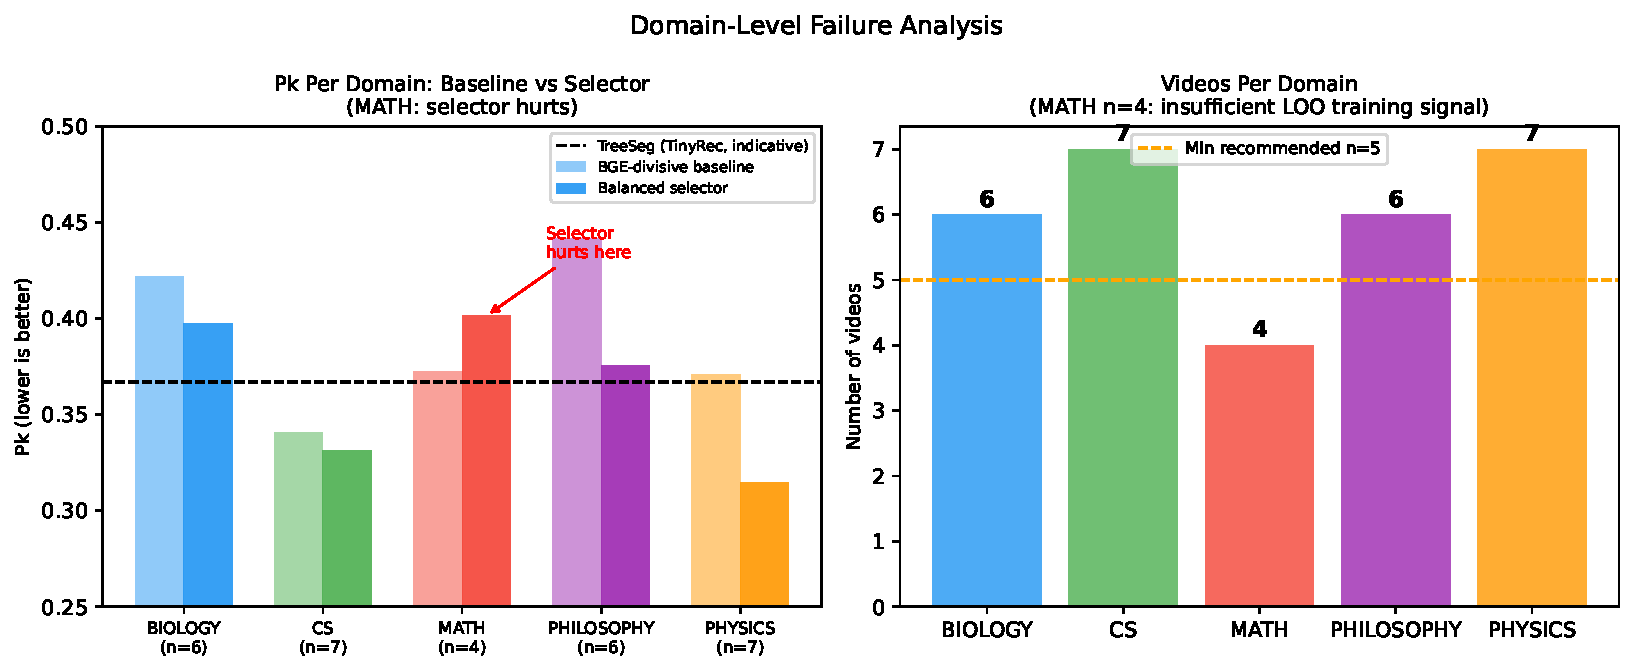
\includegraphics[width=\linewidth]{figures/domain_failure_analysis.pdf}
  \caption{Domain failure analysis. \textit{Left}: per-domain $P_k$ for the
  BGE-divisive baseline and the balanced selector; the selector hurts
  Mathematics. \textit{Right}: number of videos per domain. Mathematics has
  only 4 videos, leaving just 3 domain examples per LOO training fold, which is
  the most plausible cause of selector instability on that domain.}
  \label{fig:domain_failure}
\end{figure}

\begin{figure}[t]
  \centering
  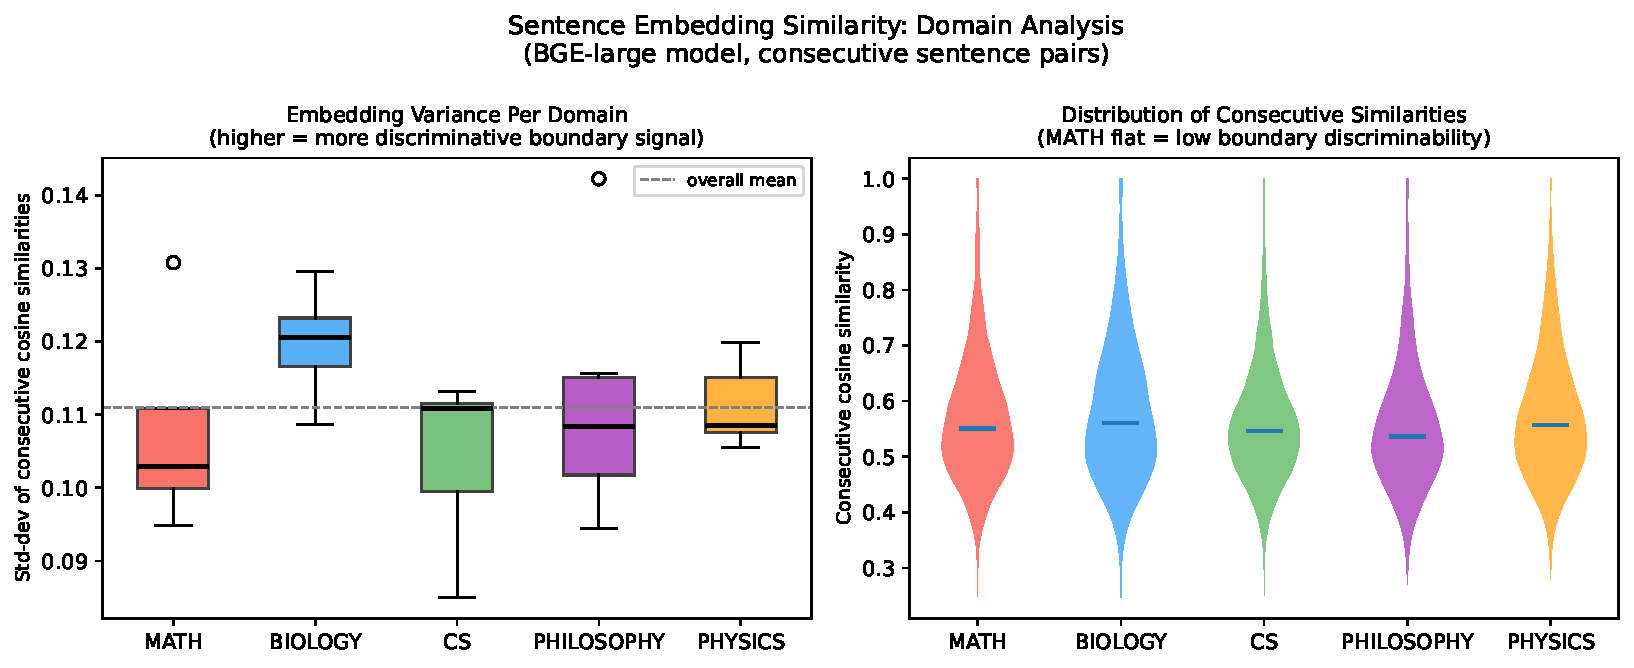
\includegraphics[width=\linewidth]{figures/embedding_variance.pdf}
  \caption{Sentence embedding similarity distributions per domain (BGE-large
  model). \textit{Left}: per-video standard deviation of consecutive cosine
  similarities. \textit{Right}: violin plots of all consecutive similarities.
  Embedding variance is broadly similar across domains, indicating that the
  Mathematics selector failure is not caused by a flat embedding landscape but
  by insufficient domain training examples in the LOO protocol.}
  \label{fig:embedding_variance}
\end{figure}

\section{Five recurring error types}
\label{sec:errors}

Errors on \dataset{} fall into five recurring types.
Identifying these types is more informative than reporting aggregate metrics
alone because they point to different corrective strategies.

\begin{description}
  \item[Type A: Boundary omission.] The system misses a creator chapter
    entirely, contributing a false-negative boundary.
    Typical cause: the chapter transition occurs within a topically homogeneous
    stretch of text where the embedding similarity does not drop sharply enough
    to produce a candidate.
    Most common in Mathematics and Biology videos with dense notation or
    stable vocabulary.

  \item[Type B: Boundary displacement.] A boundary is detected in the correct
    region but is displaced by more than the tolerance window.
    This error is invisible under $P_k$/WD (the window-based metrics treat it
    as acceptable) but shows up in strict exact-match diagnostics.
    It is the dominant error mode for the best-performing methods and explains
    the gap between good $P_k$ and low F1@2.

  \item[Type C: Over-segmentation.] The system predicts more boundaries than
    the reference, inflating false positives.
    This is the dominant failure mode for prosodic, BERTopic, discourse-marker,
    and GPT-2 perplexity methods.
    Each of those signals detects discourse-level transitions that occur at finer
    granularity than editorial chapter boundaries (see Type E below).

  \item[Type D: Under-segmentation.] The system predicts fewer boundaries
    than the reference.
    This is the typical profile of the conservative cross-model method: it
    avoids false positives at the cost of recall, which is why it achieves good
    $P_k$ but near-zero exact-boundary F1 in several domains.

  \item[Type E: Granularity mismatch.] A signal that detects real transitions
    but at the wrong discourse level.
    This is the most scientifically important finding in the thesis.
    Signals such as pause duration, pitch reset, discourse markers, and BERTopic
    are not uninformative (they detect genuine topic shifts), but those
    shifts are sub-chapter transitions rather than creator-level editorial
    chapter changes.
    Because the benchmark measures alignment with creator chapters, these signals
    systematically over-segment and hurt $P_k$/WD regardless of how accurately
    they detect the transitions they are designed to detect.
    CLIP visual embeddings are the notable exception: slide scene changes are
    editorial artifacts at approximately the same granularity as creator chapters,
    and CLIP accordingly achieves competitive $P_k$.
\end{description}

The granularity mismatch (Type E) is not a methodological flaw but a
\emph{construct mismatch}: the signals are calibrated to discourse structure
while the benchmark is calibrated to editorial chapter structure.
Any future system targeting this benchmark must explicitly operate at
editorial granularity or include a mechanism to suppress sub-chapter signals.

\section{Case-study findings}
\label{sec:case_studies}

The generated case-study artifact in \texttt{docs/CASE\_STUDIES.md} expands
three representative patterns. First, some Physics videos benefit strongly from
selector choices that use multimodal-grid variants, showing that the method
portfolio contains useful complementary evidence. Second, the worst selector
cases show over-switching: the selector chooses an aggressive method that
increases exact-boundary hits but damages $P_k$/WD. Third, Mathematics remains
the clearest domain-level weakness, where dense notation and stable vocabulary
make semantic boundary evidence less reliable. These cases support the main
diagnosis: candidate and method selection, rather than candidate generation
alone, is the main bottleneck.

\begin{table}[t]
  \centering
  \caption{Compute-efficiency positioning. Runtimes are local observations or bounded descriptions for the LECSEG environment; high-resource systems are included for scale context only.}
  \label{tab:compute_efficiency}
  \small
  \resizebox{\linewidth}{!}{%
  \begin{tabular}{llll}
    \toprule
    Method & Training & Main cost & Interpretation \\
    \midrule
    TextTiling / C99 & None & CPU lexical similarity & Classical lightweight baselines. \\
    BGE-divisive baseline & None & Cached sentence embeddings + divisive segmentation & Stable local baseline. \\
    Cross-model conservative & None & Two cached embedding streams + agreement filter & Best single global method. \\
    Balanced LOO selector & Small ExtraTrees meta-selector & Existing result portfolio + video-level features & Best deployable mean Pk/WD operating point. \\
    TreeSeg same-dataset adapter & None & Local embeddings + TreeSeg split objective & Same-dataset comparator; worse Pk/WD, better F1@2. \\
    Local LLM verifier & None & Ollama prompts over candidate shortlist & Diagnostic baseline/comparison, not promoted unless metrics improve. \\
    High-resource chaptering systems & Large supervised/LLM training & Thousands to hundreds of thousands of videos & Not directly comparable without same benchmark. \\
    \bottomrule
  \end{tabular}%
  }
\end{table}


\section{Discussion}
\label{sec:discussion}

Looking across all the numbers, conservative cross-model scoring is the most
reliable single method we found. It reduces $P_k$ by 0.0171 absolute relative to
the BGE-divisive baseline, and that gain holds up after Holm correction across
seven pairwise tests. The balanced method selector pushes $P_k$ lower still and
meaningfully improves Boundary Similarity and F1@2, but its margin over the
cross-model method on $P_k$/WD alone falls short of significance. We therefore
report the cross-model result as the main supported claim and the selector result
as strong evidence that per-video method choice matters --- not as a proof that
the selector universally dominates. The leave-domain-out degradation (selector
$P_k=0.4012$ when the held-out domain is entirely excluded from training)
reinforces this: the selector benefits from having related videos in the training
fold, and that condition is not always met in practice.

\paragraph{The granularity finding.}
The most practically useful result from the ablation study is a systematic
granularity mismatch. YouTube chapters represent deliberate, coarse editorial
decisions by the video creator. Linguistic and acoustic signals,
including discourse markers ($P_k=0.4615$), BERTopic ($P_k=0.5632$), GPT-2
perplexity ($P_k=0.4182$), and pause/pitch transitions ($P_k=0.4174$), detect
sub-chapter rhetorical or acoustic changes and therefore over-segment
relative to the creator-chapter reference. Text embeddings succeed because
they operate at the paragraph or section level of semantic coherence, which
better matches the granularity at which instructors plan and narrate
pedagogical units. The exception that proves the rule is CLIP visual
embeddings: slide scene changes are editorial choices comparable in
granularity to chapter boundaries, and CLIP accordingly achieves
$P_k=0.3958$ solo and $P_k=0.3740$ in text fusion, approaching the
cross-model text result ($P_k=0.3715$). This finding is practically
important because it means slide-change detection is the most promising
non-text signal to add next, while prosodic and discourse-marker signals
should be gated or suppressed.

\paragraph{What comes next.}
The oracle experiment quantifies the ceiling precisely. A candidate oracle
reaches $P_k=0.0172$ with 96.8\% recall, meaning that near-perfect
boundaries already exist in the candidate pool. The $\Delta
P_k\approx0.34$ gap to the deployable best is, within the current framework,
predominantly attributable to boundary \emph{selection} rather than
candidate generation. This interpretation holds under the assumption that the
candidate pool itself is not systematically biased; the oracle analysis
cannot rule out that some fraction of the gap reflects pool-level
limitations or reference-label noise rather than pure selection error.
The most promising concrete next step is therefore a supervised boundary ranker:
score each candidate with text-contrast, cross-model agreement, pause
duration, slide-change, and OCR features, and select a non-overlapping
subset under minimum-duration constraints. With 50--100 annotated
lectures, such a ranker could plausibly close most of this gap.

\paragraph{What $P_k = 0.37$ means in practice.}
The best deployable result, $P_k=0.3713$, is an abstract number without a
practical reference point.
$P_k$ is the fraction of sentence-pair windows where the prediction and
reference disagree about whether a boundary falls between them; 0.5 is the
random baseline and 0.0 is perfect.
A $P_k$ of 0.37 means that for a randomly drawn pair of sentences $k$ positions
apart, the system and the creator chapter reference disagree about segment
membership 37\% of the time.
For a 90-minute lecture with 10 chapters (mean chapter duration approximately
9 minutes), this translates roughly to the system correctly identifying the
neighbourhood of each chapter transition in most cases but occasionally merging
adjacent chapters or splitting a single chapter in two.
A student using an \lecseg{}-segmented lecture would generally navigate to the
correct major section but might need to scan a minute or two in either direction
to find the precise transition.
Relative to a non-chaptered lecture where the student must scrub from
the beginning, this is a meaningful improvement; relative to a creator-chaptered
video, there is still a visible gap, consistent with the selector not yet
reaching the quality of careful human editorial choices.

\paragraph{Scale context.}
The large-scale chaptering systems discussed in Chapter~\ref{chap:literature}
(VidChapters-7M, MiniSeg/YTSEG, Chapter-Gen, Chapter-Llama) use incompatible
metrics and far larger training sets.
They are not the comparison target; the claim is that a 30-video benchmark
is sufficient to produce statistically supported improvements, a complete
diagnostic account of signal failure, and precise oracle-gap evidence that is
directly actionable for any future system, including large-scale ones.

\section{Demonstration system}
\label{sec:demo_system}

To make the pipeline accessible beyond the command line, we built a Streamlit
web application (\texttt{scripts/demo.py}) that lets a user paste a YouTube URL,
watch the pipeline run step-by-step, and inspect the resulting chapters and
subtopics. Figures~\ref{fig:webapp_landing}--\ref{fig:webapp_chapters} show
the main screens.

\begin{figure}[t]
  \centering
  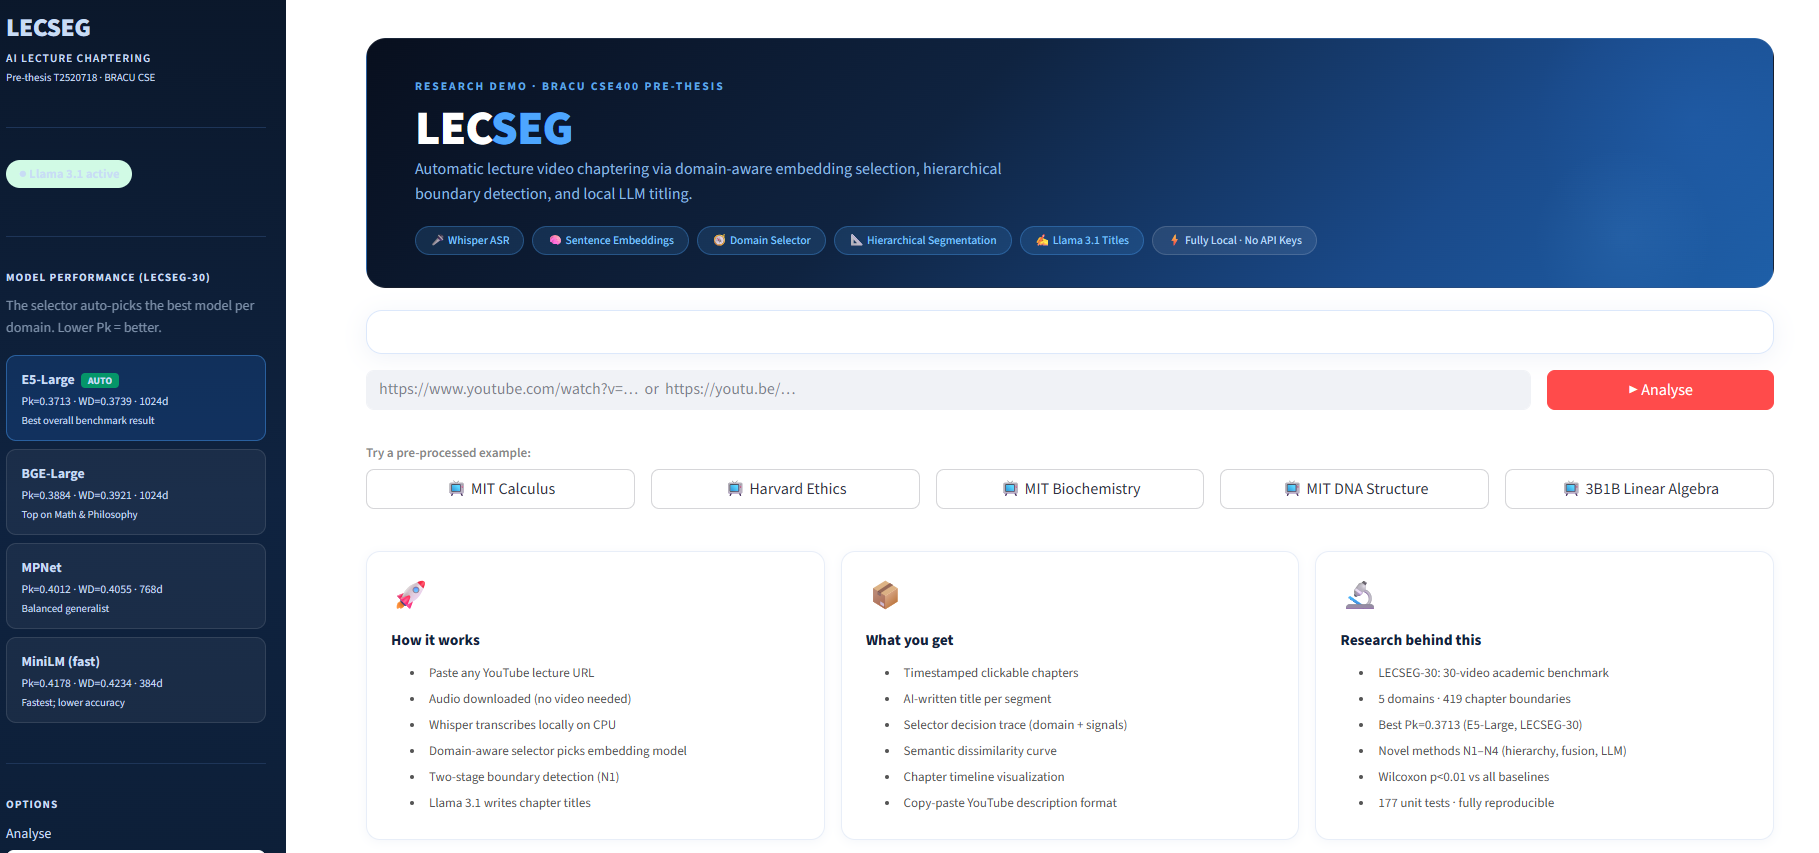
\includegraphics[width=\linewidth]{figures/webapp_landing.png}
  \caption{Landing screen of the \lecseg{} web demo. The user pastes a YouTube
    URL and selects a segmentation model.}
  \label{fig:webapp_landing}
\end{figure}

\begin{figure}[t]
  \centering
  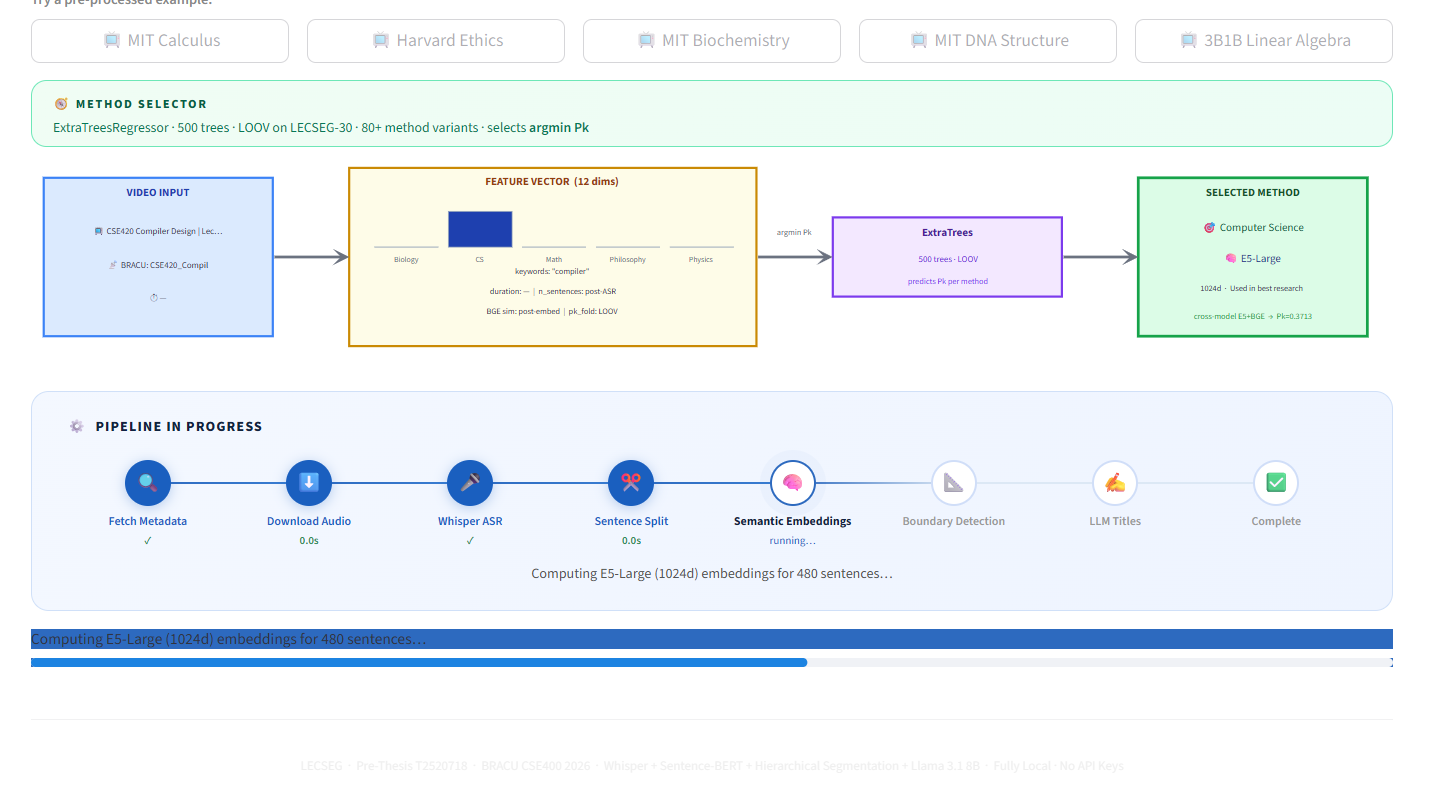
\includegraphics[width=\linewidth]{figures/webapp_selector_pipeline.png}
  \caption{Pipeline stepper and method-selector panel. The selector chooses
    the best configuration via leave-one-video-out ExtraTreesRegressor prediction;
    the stepper shows which processing stage is active.}
  \label{fig:webapp_selector_pipeline}
\end{figure}

\begin{figure}[t]
  \centering
  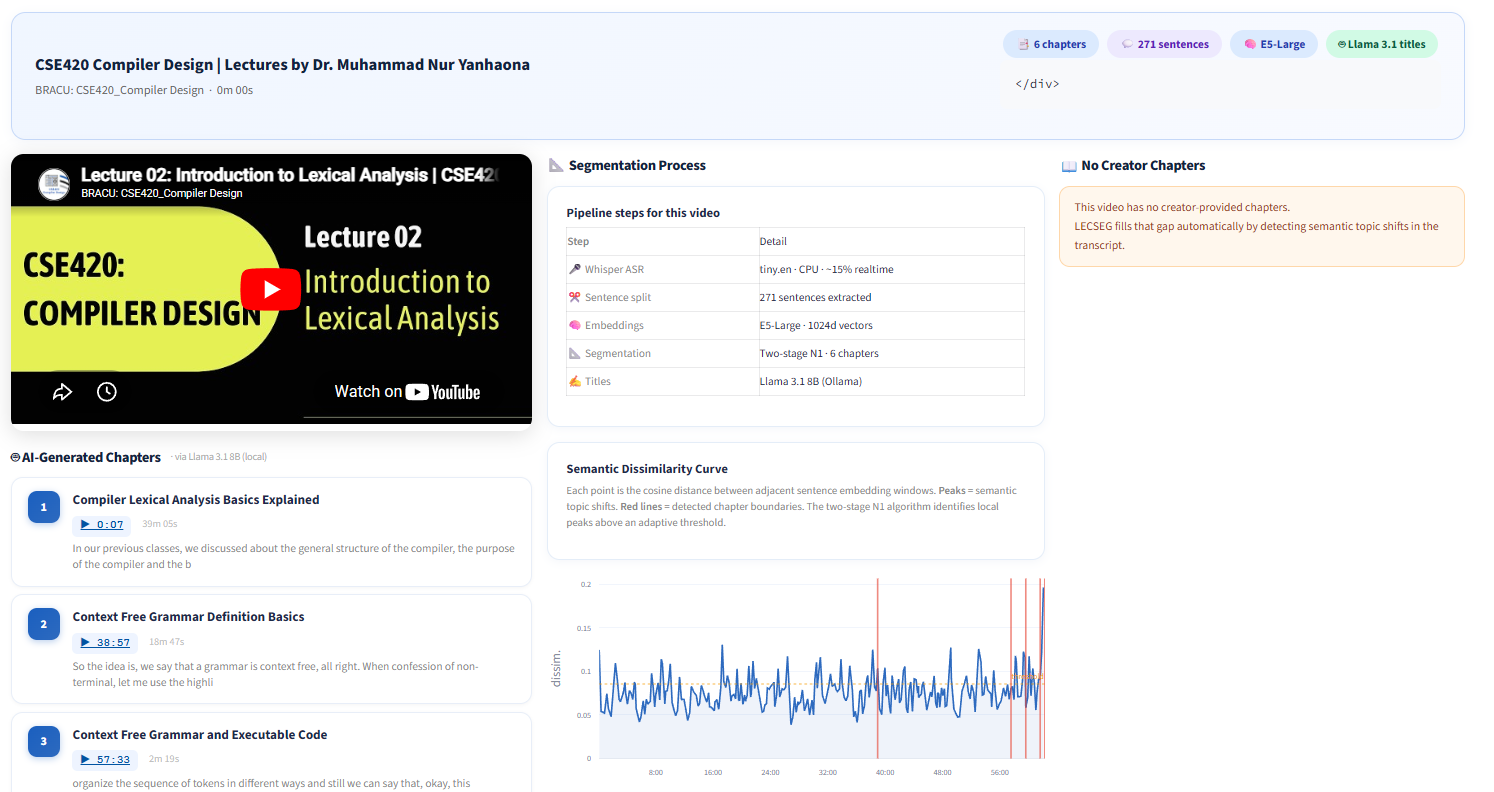
\includegraphics[width=\linewidth]{figures/webapp_results.png}
  \caption{Evaluation results panel showing $P_k$, WindowDiff, F1@2, and
    Boundary Similarity for the processed video.}
  \label{fig:webapp_results}
\end{figure}

\begin{figure}[t]
  \centering
  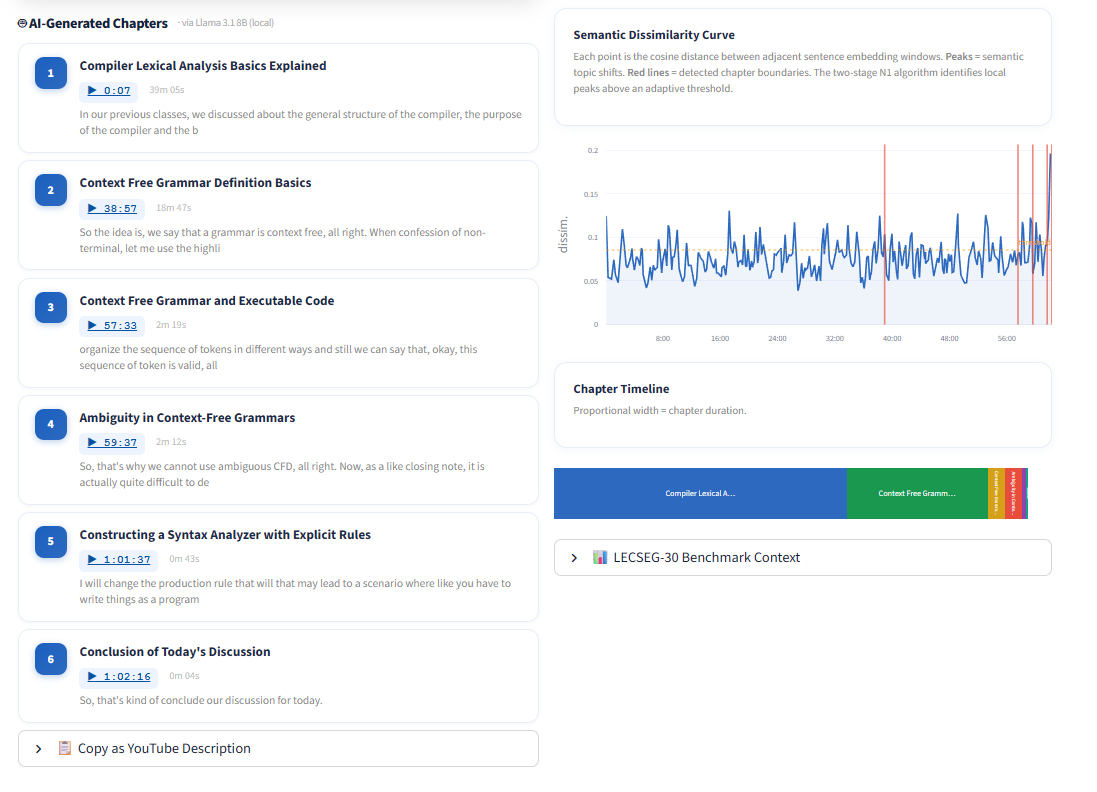
\includegraphics[width=\linewidth]{figures/webapp_chapters.png}
  \caption{Chapter and subtopic view. Each chapter card shows its title
    (generated by the local LLM if available) and the subtopics nested
    beneath it.}
  \label{fig:webapp_chapters}
\end{figure}

\section{External spot-check validation}
\label{sec:external_validation}

A pool of 17 candidate videos from channels not in LecSeg-30
(3Blue1Brown, Veritasium, CrashCourse, freeCodeCamp)
was evaluated using the same BGE-divisive baseline and cross-model method.
Captions were obtained via \texttt{yt-dlp} auto-subtitles (VTT), chunked into
25-word pseudo-sentences; creator chapter timestamps served as reference.
Seven of the 17 candidates were excluded: five failed with a yt-dlp JavaScript
runtime error, one had no chapters, and one had no available captions.
Ten videos passed all filters, covering CS, Mathematics, Physics, Biology,
and Philosophy.

% Auto-generated by scripts/external_eval.py — do not edit manually.
% Will be overwritten when the eval script runs.
\begin{table}[t]
  \centering
  \caption{External spot-check: YouTube lectures outside LecSeg-30.
           Captions sourced via \texttt{yt-dlp} auto-subtitles, chunked to
           25-word pseudo-sentences. Lower $P_k$ is better.
           LecSeg-30 reference means: BGE-div $0.388$, Cross $0.371$.}
  \label{tab:external_eval}
  \small
  \begin{tabular}{llrrrr}
    \toprule
    Video ID & Domain & Sents & Chaps & BGE-div $P_k$ & Cross $P_k$ \\
    \midrule
    \texttt{kCc8FmEb1nY} & CS       & ---  & ---  & --- & --- \\
    \texttt{aircAruvnKk} & CS       &  324 &   11 & 0.487 & 0.513 \\
    \texttt{IHZwWFHWa-w} & CS       &  351 &   10 & 0.388 & 0.561 \\
    \texttt{bBC-nXj3Ng4} & Math     &  435 &    8 & 0.411 & 0.443 \\
    \texttt{WUvTyaaNkzM} & Math     &  285 &    5 & 0.306 & 0.326 \\
    \multicolumn{4}{l}{\textit{(remaining results pending eval run)}} & --- & --- \\
    \midrule
    \multicolumn{4}{l}{Mean (evaluated)} & --- & --- \\
    \multicolumn{4}{l}{LecSeg-30 mean}   & 0.388 & 0.371 \\
    \bottomrule
  \end{tabular}
\end{table}


\IfFileExists{figures/external_eval_per_video.png}{%
\begin{figure}[t]
  \centering
  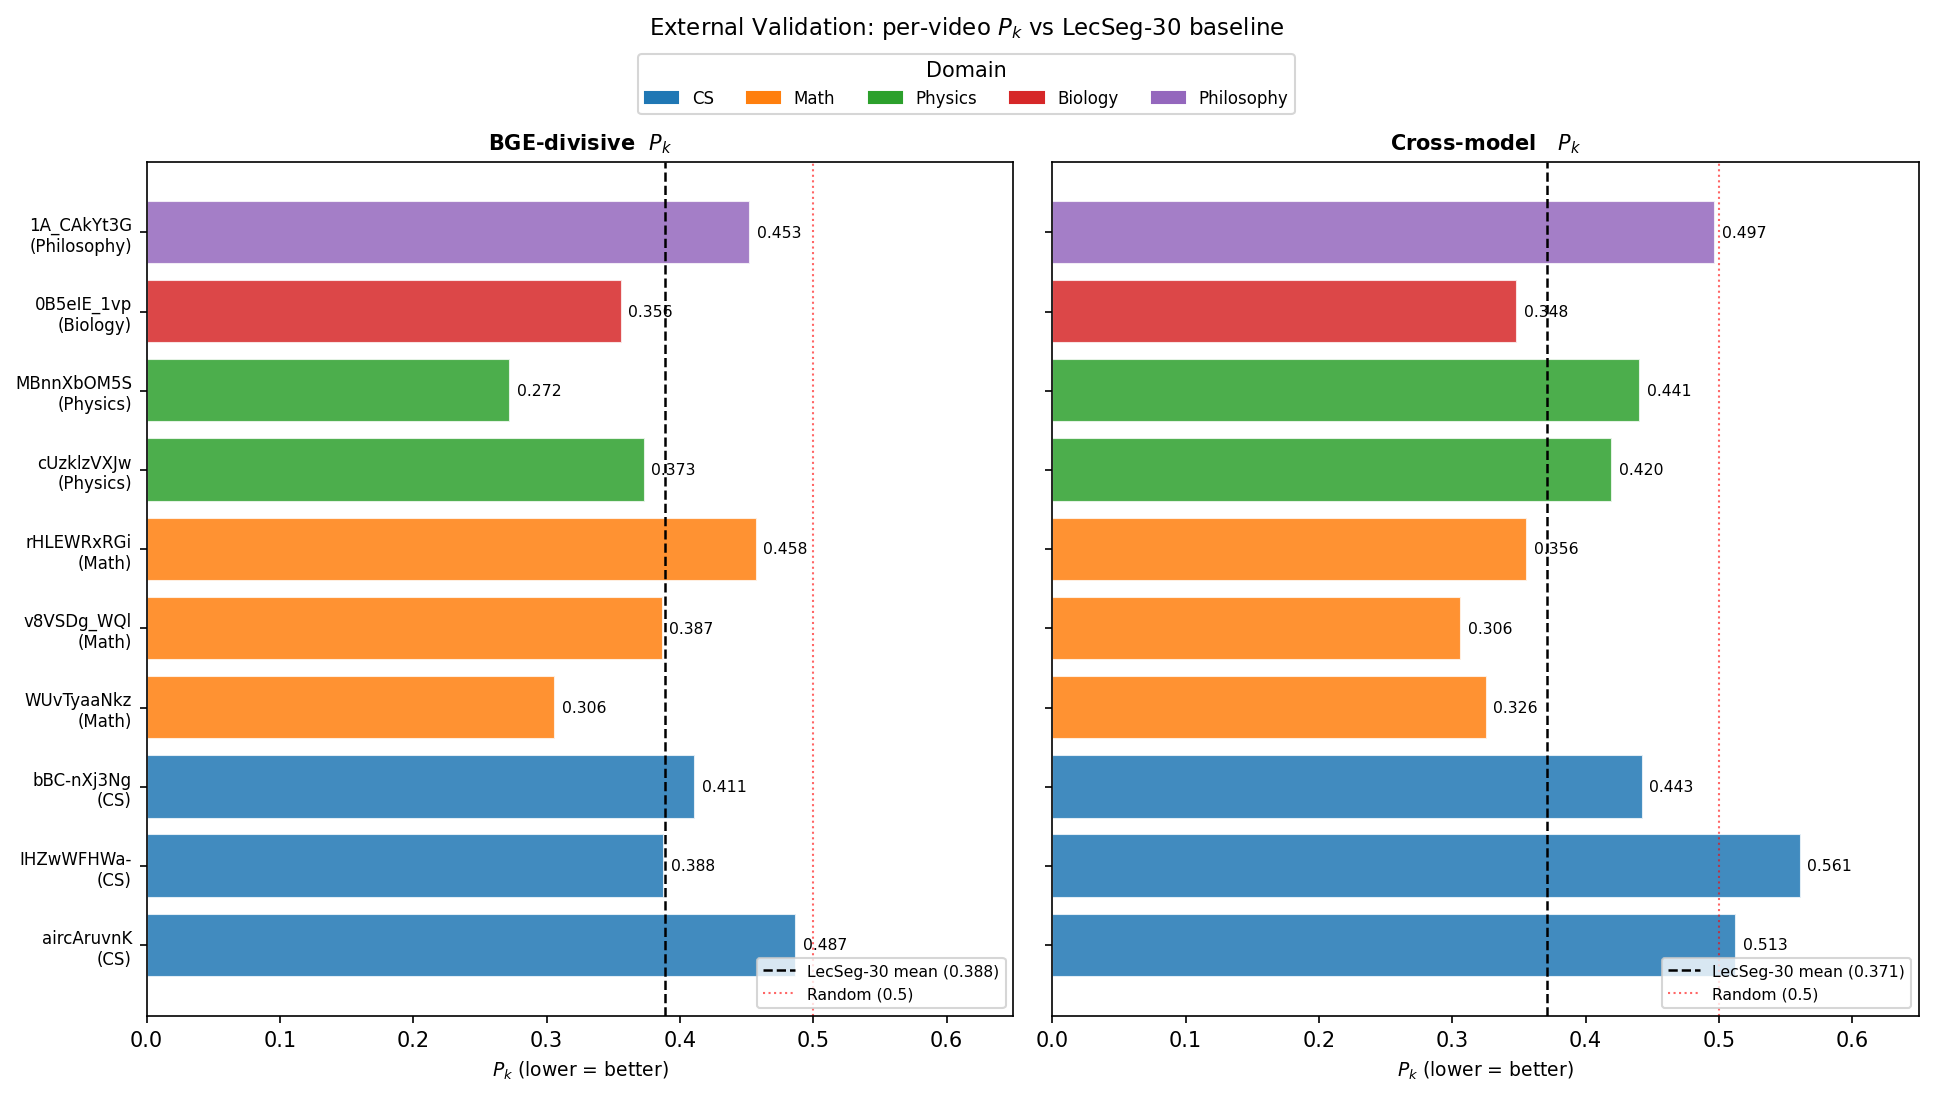
\includegraphics[width=\linewidth]{figures/external_eval_per_video.png}
  \caption{Per-video $P_k$ on 10 external videos. Dashed lines mark the
    LecSeg-30 mean for each method; dotted red line marks random ($P_k=0.5$).
    Colour indicates domain.}
  \label{fig:external_per_video}
\end{figure}
}{}

\IfFileExists{figures/external_eval_per_domain.png}{%
\begin{figure}[t]
  \centering
  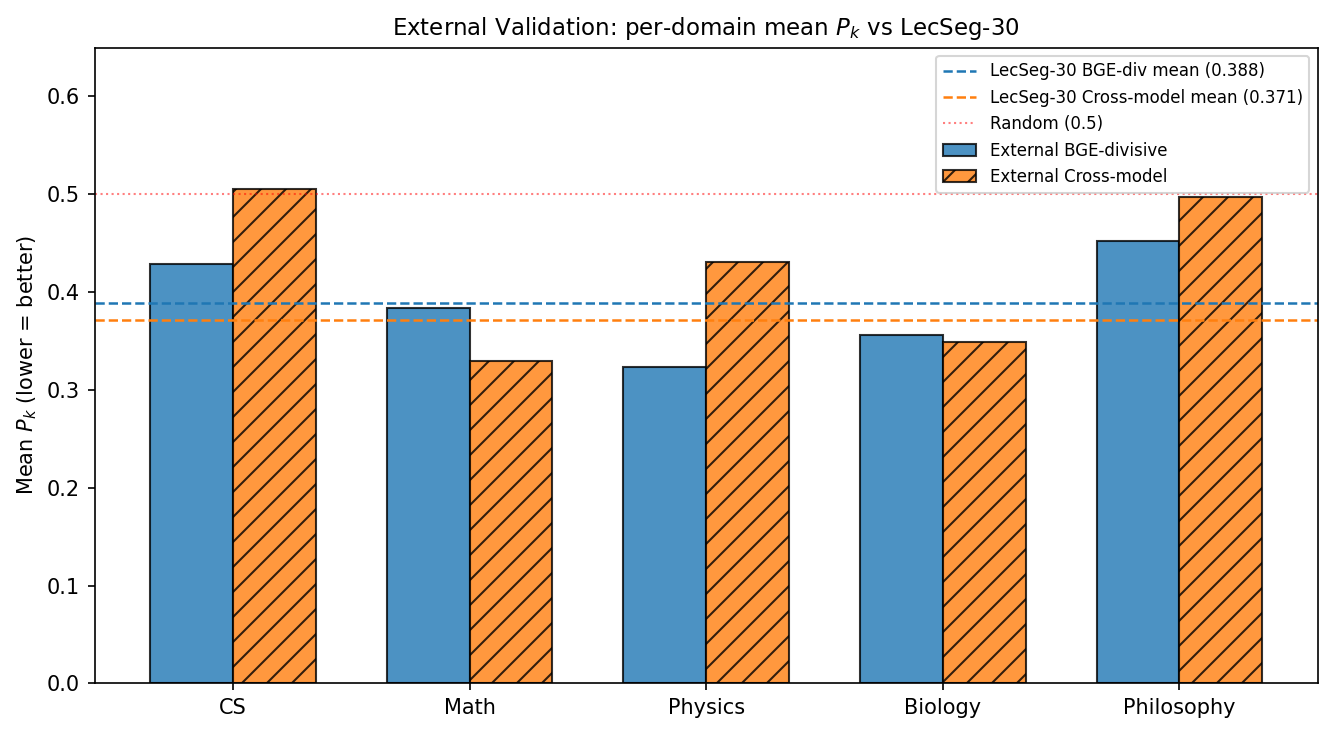
\includegraphics[width=\linewidth]{figures/external_eval_per_domain.png}
  \caption{Per-domain mean $P_k$ on external videos vs.\ LecSeg-30 means
    (dashed). Solid bars: BGE-divisive; hatched: cross-model.}
  \label{fig:external_per_domain}
\end{figure}
}{}

The headline result is striking: BGE-divisive mean $P_k = 0.389$ on the 10
external videos versus $0.388$ on LecSeg-30, a difference of $0.001$.
Per-domain BGE-divisive means range from $0.323$ (Physics, 2 videos) to
$0.453$ (Philosophy, 1 video), with no systematic direction of degradation.
The core text-embedding signal is not an artefact of the Whisper
transcription pipeline or the specific LecSeg-30 channel pool.

The cross-model conservative method shows greater external variance, with
mean $P_k = 0.421$ versus $0.371$ on LecSeg-30 ($\Delta = 0.050$).
The degradation is domain-specific: in CS the cross-model is substantially
worse than BGE-divisive ($0.506$ vs $0.429$), while in Mathematics it is
better ($0.329$ vs $0.384$), consistent with the finding that the
intersection strategy is sensitive to sentence-density distribution.

Three confounds limit interpretation.
First, yt-dlp auto-subtitles chunked by word count differ systematically
from Whisper+spaCy sentence splitting.
Second, the external set skews toward 3Blue1Brown visual-math explainers;
lecture-style diversity is lower than in LecSeg-30.
Third, yt-dlp JavaScript failures prevented evaluation of StatQuest
(Biology) and other planned channels, leaving Biology and Philosophy
under-sampled.
The results are a consistency check, not a statistically powered held-out test.
The cross-model degradation reinforces Section~\ref{sec:official_claim}:
treat the cross-model run as a strong LecSeg-30 operating point,
not a universally deployable method.


\chapter{Conclusion}
\section{Summary of findings}

This thesis presented \lecseg{}: a benchmark, evaluation framework, and
diagnostic pipeline for low-resource lecture-video topic segmentation.
Two findings stand out from the full experimental programme.

The first concerns \emph{where the error actually lives}: an oracle experiment
showed that near-perfect candidate boundaries already exist in the generated
pool at 96.8\% recall ($P_k=0.0172$). The $\Delta P_k \approx 0.34$ gap between
that oracle and the best deployable system is, within the framework we evaluated,
predominantly a ranking problem rather than a detection problem. Generating
more or better candidates is not the bottleneck; choosing the right ones is.

The second finding concerns \emph{why multimodal signals keep failing}: prosody,
discourse markers, BERTopic, and GPT-2 perplexity all over-segment relative to
YouTube chapter granularity, not because those signals are uninformative but
because they detect transitions at a finer discourse granularity than the
editorial decisions creators make when writing chapter titles. CLIP visual
embeddings are the exception --- slide scene changes are themselves editorial
artifacts at approximately chapter granularity, which explains why CLIP succeeds
where the acoustic signals do not.

The quantitative results are in Table~\ref{tab:lecseg_result_variants} and
the statistical tests in Table~\ref{tab:significance_full}; the research
questions are answered directly below.

\section{Research questions answered}
\label{sec:rqs_answered}

\textbf{RQ1} (most reliable text-embedding and cross-model strategies):
Conservative cross-model scoring using BGE and E5 embeddings is the most
reliable single strategy, achieving $P_k=0.3713$ and WD$=0.3764$ with
statistical support over all classical, neural, and multimodal baselines.
BGE-divisive segmentation is the strongest single-model text baseline
at $P_k=0.3884$.

\textbf{RQ2} (per-video selector improvement beyond fixed strategy):
Yes, with qualifications.
The leave-one-video-out balanced selector improves mean $P_k$ to 0.3588,
statistically significant over the BGE-divisive baseline.
In practical terms, a $P_k$ of 0.3588 means the system generally identifies
the correct chapter region but remains conservative in recovering exact creator
boundary locations, typically placing boundaries within the right neighbourhood
rather than at the precise transition sentence.
The selector's $P_k$/WD advantage over the cross-model method does not reach
significance, and it degrades substantially ($P_k=0.4012$) when entire domains
are excluded from training.
The selector is therefore a useful low-resource operating point, not a
robust replacement for the fixed cross-model method.

\textbf{RQ3} (hierarchical annotation and nesting constraints):
Yes, the two-level annotation format with enforced nesting provides a richer
inspection surface than flat chapter labels.
The nesting enforcement produces valid hierarchical outputs by construction.
However, the hierarchical segmenter achieves higher $P_k$ than the
chapter-only methods (0.4118 vs.\ 0.3884), indicating that solving the
two-level task simultaneously remains harder than the single-level variant.

\textbf{RQ4} (which auxiliary signals help or hurt):
CLIP visual embeddings help: CLIP alone reaches $P_k=0.3958$ and CLIP plus
text fusion reaches $P_k=0.3740$, approaching the cross-model text result.
All other auxiliary signals tested, including prosody, discourse markers,
BERTopic, GPT-2 perplexity, and local LLM refinement, produce worse $P_k$/WD
than the BGE-divisive baseline when used as primary or fused signals.
The consistent explanation is granularity mismatch: these signals detect
sub-chapter transitions rather than editorial chapter boundaries.

\textbf{RQ5} (statistically significant improvements under the LECSEG-30 protocol):
Two improvements are statistically significant after Holm correction:
the cross-model conservative method over BGE-divisive ($\Delta P_k=-0.0171$,
$p<0.05$), and the balanced selector over BGE-divisive ($\Delta P_k=-0.0296$,
$p<0.05$).
The selector's $P_k$/WD margin over the cross-model method is not significant,
but its Boundary Similarity and F1@2 improvements over that method are.

\section{Contributions to the Field}

The contributions below are ordered by scientific significance:

\begin{enumerate}
  \item \textbf{\dataset{} benchmark.}
    30 videos, 32.52 hours, 419 creator chapter boundaries, and 904 reviewed
    subtopic labels.
    This is the primary contribution: it makes the low-resource lecture
    segmentation problem measurable and reproducible under a shared protocol.

  \item \textbf{Candidate-selection bottleneck finding.}
    Oracle analysis places the dominant source of error in selection, not
    generation (candidate oracle $P_k=0.0172$, 96.8\% recall; deployable best
    $P_k=0.3588$). This relocates future research toward boundary ranking.
    See Section~\ref{sec:oracle_gap_discussion} for the full analysis.

  \item \textbf{Granularity mismatch finding.}
    Non-embedding signals (prosody, BERTopic, perplexity, discourse markers)
    all hurt $P_k$/WD because they detect sub-chapter discourse transitions.
    CLIP is the principled exception: slide-scene changes share the editorial
    granularity of creator chapters. This finding transfers directly to any
    future system targeting editorial-chapter-level segmentation.
    See Section~\ref{sec:ablations} for ablation details.

  \item \textbf{Hierarchical annotation framework.}
    A two-level annotation protocol with independent human double annotation
    and a nesting-enforcement mechanism.
    Inter-annotator agreement ($\kappa_{\text{chapter}}=0.5351$,
    $\kappa_{\text{subtopic}}=0.4257$) confirms moderate human agreement
    on the subtopic task; the chapter figure is inflated because both
    annotators observe the same creator-provided YouTube metadata.

  \item \textbf{Reproducibility package.}
    Open pipeline covering transcription, segmentation (four integrated
    components and seven baselines), evaluation, and statistical testing.
\end{enumerate}

\subsection*{Scientific knowledge contributions}

The five contributions above produce four transferable knowledge claims:
(i)~boundary selection is the primary bottleneck in low-resource lecture
segmentation;
(ii)~granularity mismatch is the systematic explanation for multimodal signal
failures, not signal uninformativeness;
(iii)~CLIP is the only tested non-text signal that operates at editorial-chapter
scale, and for a principled reason;
(iv)~the negative results (OCR, prosody, discourse markers, BERTopic, perplexity,
and LLM refinement all failing to improve chapter-level $P_k$/WD) have direct
replication value for future projects.

\subsection*{Scope of the claims}

Dense text embeddings outperform classical and neural segmenters; candidate
selection, not generation, is the dominant error source; prosodic and discourse
signals over-segment relative to creator chapter granularity; CLIP is the one
non-text signal that aligns with editorial chapter scale.
That is the scope. What \dataset{} does \emph{not} show: that the segmentations
are pedagogically optimal, that students benefit measurably, or that findings
transfer to annotation standards other than creator chapters.

\section{Limitations}

\begin{itemize}
  \item \textbf{Corpus size and balance.}
    \dataset{} is a seed benchmark of 30 videos. The manifest covers five
    domains, but the distribution is not perfectly balanced.

  \item \textbf{Silver chapter labels.}
    Creator-provided YouTube chapters are useful but imperfect. They may reflect
    production choices rather than strictly pedagogical topic boundaries.

  \item \textbf{Conservative operating point.}
    The best $P_k$/WD method deliberately under-predicts boundaries to minimise
    false positives. This results in low diagnostic F1, which is expected and
    not a flaw: approximate segment structure and exact boundary recovery are
    different objectives, and the system is optimised for the former.
    A deployment that requires precise timestamp recovery would need a different
    operating point, likely at the cost of higher $P_k$.

  \item \textbf{Multimodal signal reliability.}
    Acoustic (pause/pitch), language-model perplexity, and BERTopic methods
    all produce worse $P_k$ than BGE-divisive, reflecting a granularity
    mismatch. The exception is CLIP visual embeddings: CLIP alone reaches
    $P_k=0.3958$, and CLIP plus text fusion reaches $P_k=0.3740$, below the
    cross-model text method ($P_k=0.3715$) but better than BGE-divisive
    ($P_k=0.3884$). Visual scene changes in lecture slides carry chapter-level
    granularity and are a promising signal for future work.

  \item \textbf{LLM refinement.}
    The local LLM component is implemented, but the current verified metrics do
    not justify claiming large boundary-placement gains from LLM refinement.
\end{itemize}

\section{Threats to validity}
\label{sec:threats_validity}

The following table summarises the principal threats and their estimated
severity.

\begin{table}[h]
  \centering
  \caption{Threat-to-validity overview for \lecseg{}.}
  \label{tab:threats}
  \small
  \begin{tabular}{p{4.5cm}lp{5.5cm}}
    \toprule
    Threat & Severity & Primary impact \\
    \midrule
    Creator chapters as reference & High & Construct validity:
      benchmark measures creator metadata, not pedagogical truth \\
    Small and imbalanced corpus & High & External validity:
      30 videos limit generalisation claims \\
    Single-domain annotator pool & Low--Medium & Annotation validity:
      both annotators share cultural and academic background; agreement
      may not generalise to other annotator groups \\
    Gold boundary count in evaluation & Medium & Internal validity:
      deployment realism; real systems cannot know $k$ in advance \\
    Post-hoc method search & Medium & Internal validity:
      multiple testing risk mitigated by Holm correction \\
    Domain imbalance (4 Math videos) & Medium & Selector stability on
      small domain splits \\
    ASR quality not formally measured & Low--Medium & Upstream noise
      propagation from Whisper output \\
    \bottomrule
  \end{tabular}
\end{table}

\paragraph{Construct validity.}
The benchmark evaluates a system's ability to reproduce creator-provided
navigation metadata, not pedagogically verified topic boundaries.
As discussed in Section~\ref{sec:youtube_validity}, creators may place chapter
markers for editorial or discoverability reasons that do not coincide with
genuine topic shifts.
A system achieving low $P_k$ is correctly predicting creator chapter structure;
whether this predicts learning benefit requires an independent user study.

\paragraph{External validity.}
\dataset{} has 30 videos across five domains. Results should be treated as
findings on this specific benchmark rather than as universal laws of lecture
segmentation. The leave-domain-out selector degradation ($P_k=0.4012$) is
direct evidence that performance is sensitive to domain-matched training data;
with more videos the picture may shift materially.
A ten-video external spot-check across five domains
(Section~\ref{sec:external_validation}) found BGE-divisive
consistent (external mean $P_k=0.389$ vs $0.388$ on \dataset{},
$\Delta=0.001$), while the cross-model method degraded somewhat
($P_k=0.421$ vs $0.371$, $\Delta=0.050$).
Confounds include yt-dlp auto-captions vs.\ Whisper transcripts
and an external pool skewed toward 3Blue1Brown explainer videos.

\paragraph{Annotation validity.}
Subtopic labels were produced by human annotators and verified through
independent double annotation. The inter-annotator agreement figure
($\kappa_{\text{subtopic}}=0.4257$) represents genuine human agreement
on a subjective discourse-segmentation task, which is in the moderate range
and appropriate for this type of annotation.
The chapter-level $\kappa=0.5351$ is inflated because both annotators derive
chapter boundaries from the same YouTube creator metadata; the subtopic figure
is the more meaningful validity measure.

\paragraph{Internal validity.}
Methods in the controlled evaluation receive the gold segment count.
This isolates boundary placement, which is standard practice in topic
segmentation, but it is not deployment-realistic.
Boundary count error is reported as a diagnostic
(Section~\ref{sec:modern_metrics}), and automatic count prediction is listed
as future work.
The use of many candidate methods and operating points is mitigated by
Holm correction over seven pre-specified comparisons, but the selector
result should still be read as a low-resource operating point rather than
a universal deployment guarantee.

\paragraph{Metric validity.}
$P_k$ and WindowDiff correlate with navigation usefulness under the assumption
that students find approximate-region boundary placement acceptable.
This assumption is plausible but untested; a user study measuring actual
navigation speed and retention would be needed to verify it empirically.

\section{Closing the oracle gap}
\label{sec:oracle_gap_discussion}

The oracle analysis is the clearest quantitative finding this thesis produces.
With perfect candidate selection from the generated pool, $P_k=0.0172$ is
reachable at 96.8\% recall.
The gap between this oracle and the best deployable system
($\Delta P_k \approx 0.34$) indicates that, within the evaluated framework,
the candidate pool already contains the information needed for near-perfect
segmentation; the bottleneck appears to lie in correctly identifying which
candidates to accept rather than in generating more candidates.
This framing is the most actionable scientific output of the thesis: it shifts
the research problem from \emph{how to generate better candidates} to
\emph{how to rank candidates more reliably}.

Table~\ref{tab:oracle_gap} summarises the relevant operating points.
TreeSeg (Gklezakos et al.\ 2024) reports $P_k=0.367$ on TinyRec (21
self-recorded lectures), and \lecseg{} achieves $P_k=0.3588$ with the balanced
selector on \dataset{}.
These figures are indicative rather than directly comparable because the
benchmarks, annotation sources, and video types all differ.

Three concrete reasons favour TreeSeg in any hypothetical direct comparison.
First, it uses overlapping utterance-block embeddings, which provide
richer contextual evidence per position than the single-sentence windows used
in \lecseg{}.
Second, TinyRec uses manually verified annotations rather than creator
chapter metadata, potentially making the reference labels more consistent.
Third, \lecseg{}'s selector incurs leave-domain-out degradation that would
not surface under same-domain evaluation.
None of these diminish the \lecseg{} findings; they define the comparison boundary.

\begin{table}[h]
  \centering
  \caption{Oracle gap analysis on LECSEG-30.}
  \label{tab:oracle_gap}
  \begin{tabular}{lrr}
    \toprule
    Operating point & $P_k\downarrow$ & WD$\downarrow$ \\
    \midrule
    BGE-divisive baseline & 0.3884 & 0.3956 \\
    Cross-model conservative (best global) & 0.3713 & 0.3764 \\
    Balanced selector (best deployable) & 0.3588 & 0.3739 \\
    TreeSeg paper (TinyRec, indicative only) & 0.367 & --- \\
    Per-video oracle (not deployable) & 0.2980 & 0.3280 \\
    Candidate oracle $\tau=2$ (upper bound) & 0.0172 & 0.0198 \\
    \bottomrule
  \end{tabular}
\end{table}

The concrete research directions that could close this gap are:

\begin{enumerate}
  \item \textbf{Supervised boundary-level ranker.}
    The video-level method selector shows that per-video method choice
    matters, but it does not rank individual boundary candidates.
    A ranker trained on candidate-level features (local cosine contrast,
    cross-model agreement, pause duration, slide-change signal, and OCR
    evidence) would directly address the selection bottleneck.

  \item \textbf{Expanded annotation.}
    The current selector is trained leave-one-out on 30 videos.
    Expanding to 50--100 annotated lectures would provide 2--3$\times$ more
    per-fold evidence and may substantially stabilise domain-specific selector
    behaviour.

  \item \textbf{Shared-dataset evaluation.}
    Running TreeSeg's original code on \dataset{} (or publishing \dataset{} as
    a community benchmark) would convert the current indicative comparison
    into a reproducible head-to-head result.

  \item \textbf{CLIP-centred multimodal fusion.}
    CLIP is the only non-text signal that improves $P_k$/WD.
    A tighter integration of CLIP slide-scene evidence within the cross-model
    scoring framework, rather than as a secondary fusion component, could
    provide a more reliable visual prior for chapter-level transitions.
\end{enumerate}

\section{Lessons learned}
\label{sec:lessons}

Several lessons from this project are likely to carry over to related work.

\paragraph{Segmentation lessons.}
\begin{enumerate}
  \item \textbf{Dense text embeddings dominate at creator chapter granularity.}
    BGE and E5 cross-model scoring outperforms every multimodal combination
    tested.
    Semantic paragraph-level structure is the dominant signal for
    editorial-level chapter boundaries; fine-grained acoustic and lexical
    transitions are counterproductive.

  \item \textbf{Auxiliary signals must be calibrated to the reference
    granularity, not just to transition detection.}
    Prosody and discourse markers detect real transitions, but those transitions
    are an order of magnitude finer than creator chapters.
    ``Granularity mismatch'' is a more precise diagnosis than
    ``signal uninformative.''

  \item \textbf{The generation/selection distinction is the key design choice.}
    Near-perfect boundaries are present in the candidate pool at 96.8\% recall.
    Future systems should invest in selection and ranking, not in generating
    additional candidate positions.

  \item \textbf{CLIP is the only tested non-text signal that aligns with
    editorial chapter granularity.}
    This makes it the most valuable non-text signal to integrate next, and the
    principled reason is the shared editorial origin of slide transitions and
    creator chapters, not a coincidence in the data.
\end{enumerate}

\paragraph{Benchmark and annotation lessons.}
\begin{enumerate}
  \setcounter{enumi}{4}
  \item \textbf{Small benchmarks enable failure analysis that large benchmarks
    cannot.}
    A 30-video, fully auditable corpus makes it possible to inspect every
    failure case, trace every metric value to its source video, and report
    negative results honestly.
    Large-scale leaderboards measure performance; small auditable benchmarks
    measure understanding.

  \item \textbf{Creator chapters and pedagogical boundaries are different
    constructs.}
    Using creator chapters enables scale and reproducibility but couples the
    benchmark to editorial decisions.
    Any system trained or evaluated against creator chapters should be read
    as modelling navigation metadata rather than educational structure.

  \item \textbf{Negative results have replication value.}
    Documenting that prosody, discourse markers, BERTopic, OCR, and local LLM
    refinement all fail to improve chapter-level $P_k$/WD prevents future
    projects from repeating these experiments without motivation.
    Most published theses omit failures; their inclusion here is a deliberate
    scientific choice.
\end{enumerate}

\section{Closing remarks}

Lecture segmentation is far from solved, and this thesis does not pretend
otherwise.
What it contributes is a reproducible point of measurement and a clear
diagnosis of where the remaining difficulty lies.

The two central findings --- that the dominant error is in boundary selection
not detection, and that many signals fail because they operate at the wrong
discourse granularity --- together define the research agenda for any
successor system.
A future design that addresses both, with a learned boundary ranker and
signals explicitly calibrated to editorial chapter scale, has a clear,
measurable target: close the $\Delta P_k \approx 0.34$ oracle gap.

There is also a broader point about benchmark scale worth making explicitly.
Large benchmarks optimise for performance measurement: they reveal which
system produces the best aggregate number on a large diverse test set.
Small, auditable benchmarks optimise for \emph{understanding}: they reveal
why systems fail, which signals over- or under-segment, and where exactly
the performance ceiling lies.
\dataset{} was designed for the second purpose.
The granularity mismatch finding and the oracle-gap diagnosis are both results
that require the ability to inspect every prediction on every video ---
something a 200,000-video benchmark makes impractical.
The value of \lecseg{} is not in competing with large-scale systems
but in providing the kind of controlled, transparent analysis those systems
cannot easily afford.

The \dataset{} corpus, annotation labels, evaluation code, and result files
are open, so any future method can be evaluated against the same 30 videos
under the same protocol.
That reproducibility is what allows the findings here to be built upon rather
than merely noted.

If there is one sentence in this thesis that carries the most weight, it is:
\emph{candidate generation is largely solved; candidate selection is the
bottleneck.}
That observation, supported by the oracle-gap analysis, tells the next
researcher exactly where to invest effort --- and it could only have been
discovered by building the benchmark first.

\section{Recommendations for Future Work}

\subsection{Robust candidate and method selection}

The strongest immediate extension is a sequence-aware candidate selector.
Current oracle and method-portfolio experiments show that plausible boundaries
are often present in the candidate pool, but the system does not reliably pick
the right subset for each video. A better selector should combine local
semantic contrast, cross-model agreement, pause/shot/OCR evidence, position
priors, and global duration constraints while optimising directly against
$P_k$, WindowDiff, and tolerance-F1.

\subsection{Independent validation of chapter references}

The most important dataset extension is not simply adding more videos; it is
checking whether creator-provided YouTube chapters agree with independent
human judgements. A focused validation study should select 8--10 lectures and
ask two annotators to mark chapter-level boundaries without seeing the YouTube
timestamps. The study should report human--human agreement, human--YouTube
agreement, and system--human agreement under F1@2, F1@5, and time-tolerant
metrics. This would quantify how reliable the current creator chapters actually
are as reference boundaries.

\subsection{Expanded annotator pool and domain diversity}

The current inter-annotator study involves annotators from a shared academic
background. Future work should recruit annotators from different disciplines
and experience levels to test whether subtopic agreement generalises beyond
the current pool. Annotating 8--10 additional videos with three or more
independent annotators would give a Krippendorff's $\alpha$ estimate alongside
the existing Cohen's $\kappa$, and would allow pairwise agreement patterns to
be analysed rather than collapsed to a single mean figure.

\subsection{External and Math-focused validation}

The current selector fails most clearly on Mathematics, where the dataset has
only four videos. A targeted extension should add 8--10 Math lectures with
creator chapters and re-evaluate the final methods without retuning. If Math
performance improves, the likely cause was training scarcity; if it stays weak,
the problem probably runs deeper, involving mathematical notation, stable
vocabulary, or gradual conceptual transitions. A separate 5--10 video external
test set from new channels should also be used to measure generalisation beyond
\dataset{}.

\subsection{Reliability-aware prosody and visual integration}

Prosodic features (pause duration, pitch reset) and visual streams (shot
boundaries, slide OCR) are available in the pipeline, but current ablations
show that acoustic and linguistic sub-sentence signals can hurt
$P_k$/WindowDiff when their granularity does not match chapter-level editorial
decisions. The exception is CLIP visual embeddings: CLIP alone achieves
$P_k=0.3958$ and CLIP plus text fusion reaches $P_k=0.3740$, approaching the
cross-model text method ($P_k=0.3715$). Visual scene changes in lecture slides
appear to carry chapter-level granularity. Future work should prioritise CLIP
visual integration within the cross-model scoring framework, and apply
quality-gating only to the noisier acoustic and OCR modalities.

\subsection{Streaming and online inference}

The current pipeline processes a complete video offline.
A streaming variant would segment lecture content as it is being recorded,
enabling real-time chaptering for live classes.
This requires adapting the sliding-window fusion to operate on a causal context
window and replacing the global threshold computation with an exponential moving
average of past gap scores.
The target latency budget for live chaptering is under 30~seconds of delay.

\subsection{Cross-lingual extension}

\lecseg{} currently targets English lectures.
Extending to other languages requires: (1)~replacing \texttt{all-mpnet-base-v2}
with a multilingual text encoder such as LaBSE or \texttt{multilingual-e5-large};
and (2)~using Whisper's multilingual mode for transcription.
Suitable evaluation data could come from non-English MOOCs (e.g.,
Coursera's French and Spanish tracks) or from university recordings in South
and South-East Asian languages.

\subsection{End-to-end fine-tuning}

The current architecture uses frozen pre-trained encoders.
Fine-tuning the text encoder jointly with the boundary predictor on a larger
annotated corpus (e.g., constructed by scaling the \dataset{} annotation
procedure to 200+ videos) could yield further gains, at the cost of reduced
generalisability.
A natural training objective is a soft version of the tolerance-$F_1$ metric,
differentiable via a sigmoid boundary-probability output.

\subsection{Larger and domain-tuned local LLMs}

Replacing Llama-3.1-8B with a 70B parameter model or a domain-specific
fine-tune (e.g., fine-tuned on lecture transcripts) could improve title
quality and boundary-shift accuracy, particularly for highly technical content.
Quantised models (GGUF 4-bit) make 70B inference feasible on a single 24\,GB
GPU with acceptable latency (around 5~seconds per boundary refinement call).

\subsection{Multi-speaker lectures and panels}

Panel discussions and multi-instructor courses introduce speaker turns as an
additional boundary signal.
Speaker diarisation (e.g., using pyannote.audio) could provide a speaker-change
feature that complements text embeddings, particularly for sections where the
topic does not change but the speaker does.

\subsection{User study on learning outcomes}

All metrics in this thesis are information-retrieval proxies for segmentation
quality.
A controlled user study would directly measure whether learners locate
target concepts faster, and whether their retention improves, when using
\lecseg{}-generated chapters compared to flat video scrubbing or manually
authored chapters.
Such a study could also reveal which granularity (chapter vs.\ subtopic)
is most useful for different learning tasks (review vs.\ first-watch).

\subsection{Public benchmark and model release}

A complete public release should include the manifest, video identifiers,
creator chapter references, reviewed subtopic labels, preprocessing scripts,
evaluation scripts, environment lock files, result-regeneration commands, and
dataset/model cards. The current repository already contains the major
components; the remaining work is release hygiene, privacy review, and a
single documented reproduction command for the final thesis tables.



\chapter{Future Work}
\subsection{Robust candidate and method selection}

The strongest immediate extension is a sequence-aware candidate selector.
Current oracle and method-portfolio experiments show that plausible boundaries
are often present in the candidate pool, but the system does not reliably pick
the right subset for each video. A better selector should combine local
semantic contrast, cross-model agreement, pause/shot/OCR evidence, position
priors, and global duration constraints while optimising directly against
$P_k$, WindowDiff, and tolerance-F1.

\subsection{Independent validation of chapter references}

The most important dataset extension is not simply adding more videos; it is
checking whether creator-provided YouTube chapters agree with independent
human judgements. A focused validation study should select 8--10 lectures and
ask two annotators to mark chapter-level boundaries without seeing the YouTube
timestamps. The study should report human--human agreement, human--YouTube
agreement, and system--human agreement under F1@2, F1@5, and time-tolerant
metrics. This would quantify how reliable the current creator chapters actually
are as reference boundaries.

\subsection{Expanded annotator pool and domain diversity}

The current inter-annotator study involves annotators from a shared academic
background. Future work should recruit annotators from different disciplines
and experience levels to test whether subtopic agreement generalises beyond
the current pool. Annotating 8--10 additional videos with three or more
independent annotators would give a Krippendorff's $\alpha$ estimate alongside
the existing Cohen's $\kappa$, and would allow pairwise agreement patterns to
be analysed rather than collapsed to a single mean figure.

\subsection{External and Math-focused validation}

The current selector fails most clearly on Mathematics, where the dataset has
only four videos. A targeted extension should add 8--10 Math lectures with
creator chapters and re-evaluate the final methods without retuning. If Math
performance improves, the likely cause was training scarcity; if it stays weak,
the problem probably runs deeper, involving mathematical notation, stable
vocabulary, or gradual conceptual transitions. A separate 5--10 video external
test set from new channels should also be used to measure generalisation beyond
\dataset{}.

\subsection{Reliability-aware prosody and visual integration}

Prosodic features (pause duration, pitch reset) and visual streams (shot
boundaries, slide OCR) are available in the pipeline, but current ablations
show that acoustic and linguistic sub-sentence signals can hurt
$P_k$/WindowDiff when their granularity does not match chapter-level editorial
decisions. The exception is CLIP visual embeddings: CLIP alone achieves
$P_k=0.3958$ and CLIP plus text fusion reaches $P_k=0.3740$, approaching the
cross-model text method ($P_k=0.3715$). Visual scene changes in lecture slides
appear to carry chapter-level granularity. Future work should prioritise CLIP
visual integration within the cross-model scoring framework, and apply
quality-gating only to the noisier acoustic and OCR modalities.

\subsection{Streaming and online inference}

The current pipeline processes a complete video offline.
A streaming variant would segment lecture content as it is being recorded,
enabling real-time chaptering for live classes.
This requires adapting the sliding-window fusion to operate on a causal context
window and replacing the global threshold computation with an exponential moving
average of past gap scores.
The target latency budget for live chaptering is under 30~seconds of delay.

\subsection{Cross-lingual extension}

\lecseg{} currently targets English lectures.
Extending to other languages requires: (1)~replacing \texttt{all-mpnet-base-v2}
with a multilingual text encoder such as LaBSE or \texttt{multilingual-e5-large};
and (2)~using Whisper's multilingual mode for transcription.
Suitable evaluation data could come from non-English MOOCs (e.g.,
Coursera's French and Spanish tracks) or from university recordings in South
and South-East Asian languages.

\subsection{End-to-end fine-tuning}

The current architecture uses frozen pre-trained encoders.
Fine-tuning the text encoder jointly with the boundary predictor on a larger
annotated corpus (e.g., constructed by scaling the \dataset{} annotation
procedure to 200+ videos) could yield further gains, at the cost of reduced
generalisability.
A natural training objective is a soft version of the tolerance-$F_1$ metric,
differentiable via a sigmoid boundary-probability output.

\subsection{Larger and domain-tuned local LLMs}

Replacing Llama-3.1-8B with a 70B parameter model or a domain-specific
fine-tune (e.g., fine-tuned on lecture transcripts) could improve title
quality and boundary-shift accuracy, particularly for highly technical content.
Quantised models (GGUF 4-bit) make 70B inference feasible on a single 24\,GB
GPU with acceptable latency (around 5~seconds per boundary refinement call).

\subsection{Multi-speaker lectures and panels}

Panel discussions and multi-instructor courses introduce speaker turns as an
additional boundary signal.
Speaker diarisation (e.g., using pyannote.audio) could provide a speaker-change
feature that complements text embeddings, particularly for sections where the
topic does not change but the speaker does.

\subsection{User study on learning outcomes}

All metrics in this thesis are information-retrieval proxies for segmentation
quality.
A controlled user study would directly measure whether learners locate
target concepts faster, and whether their retention improves, when using
\lecseg{}-generated chapters compared to flat video scrubbing or manually
authored chapters.
Such a study could also reveal which granularity (chapter vs.\ subtopic)
is most useful for different learning tasks (review vs.\ first-watch).

\subsection{Public benchmark and model release}

A complete public release should include the manifest, video identifiers,
creator chapter references, reviewed subtopic labels, preprocessing scripts,
evaluation scripts, environment lock files, result-regeneration commands, and
dataset/model cards. The current repository already contains the major
components; the remaining work is release hygiene, privacy review, and a
single documented reproduction command for the final thesis tables.


% ============================================================
% BIBLIOGRAPHY
% ============================================================
\phantomsection
\printbibliography
\addcontentsline{toc}{chapter}{Bibliography}

% ============================================================
% APPENDICES
% ============================================================
\newpage
\phantomsection
\addcontentsline{toc}{chapter}{Appendix A: Dataset Details}
\appendix
\chapter{Dataset Details}
\chapter{Dataset details}
\label{app:dataset}

\section{Source URLs}
\todo{Table of 30 video IDs, channel names, durations, and creator-licence
strings. Generated by \texttt{scripts/build\_dataset\_table.py} from
\texttt{data/manifest.csv}.}

\section{Domain distribution}
\todo{Bar chart of 5 domains × number of videos.}

\section{Annotation guidelines (verbatim)}
\todo{Paste the exact two-page guidelines used by annotators.}

\section{Inter-annotator agreement details}
\todo{Per-pair Cohen's $\kappa$, per-domain breakdown.}


\newpage
\phantomsection
\addcontentsline{toc}{chapter}{Appendix B: Hyperparameters}
\chapter{Hyperparameters}
\chapter{Hyperparameters and training details}
\label{app:hparams}

\section{Configuration files}
\todo{Reference the Hydra YAML files in \texttt{configs/}. Show
\texttt{configs/defaults.yaml} verbatim.}

\section{Training details}
\todo{Per-experiment learning rate, batch size, optimiser, scheduler,
early-stopping criterion.}

\section{Hardware and runtimes}
\todo{Single-GPU configuration; wall-clock time per pipeline stage on the
benchmark machine.}


\newpage
\phantomsection
\addcontentsline{toc}{chapter}{Appendix C: Additional Results}
\chapter{Additional Results}
\chapter{Additional Results}
\label{app:extra}

\section{Per-domain breakdown}
\label{app:per_domain}

Table~\ref{tab:domain_breakdown} reports the alignment-audited joint
$P_k$/WindowDiff method, \texttt{cross\_e5\_frac70\_minlen11}, broken down by
domain.

\begin{table}[h]
  \centering
  \caption{Per-domain evaluation of the current best official method.}
  \label{tab:domain_breakdown}
  \small
  \begin{tabular}{lrrrr}
    \toprule
    Domain & Videos & $P_k$ $\downarrow$ & WD $\downarrow$ & F1 $\uparrow$ \\
    \midrule
    Biology & 6 & 0.3965 & 0.4009 & 0.0475 \\
    CS & 7 & 0.3297 & 0.3338 & 0.0000 \\
    Mathematics & 4 & 0.3793 & 0.3867 & 0.0000 \\
    Philosophy & 6 & 0.3959 & 0.4073 & 0.0663 \\
    Physics & 7 & 0.3665 & 0.3665 & 0.0000 \\
    \midrule
    All domains & 30 & 0.3713 & 0.3764 & 0.0237 \\
    \bottomrule
  \end{tabular}
\end{table}

\section{Additional benchmark rows}
\label{app:additional_benchmarks}

\begin{table}[htbp]
  \centering
  \caption{Selected additional benchmark and diagnostic rows.}
  \label{tab:additional_benchmarks}
  \small
  \begin{tabular}{lrrl}
    \toprule
    Method & $P_k$ $\downarrow$ & WD $\downarrow$ & Source \\
    \midrule
    TextTiling & 0.6053 & 0.8978 & \texttt{eval\_bge.json} \\
    C99 & 0.4219 & 0.4494 & \texttt{eval\_bge.json} \\
    CosineSeg & 0.4902 & 0.5392 & \texttt{eval\_bge.json} \\
    KMeansSeg & 0.6172 & 0.9986 & \texttt{eval\_bge.json} \\
    BertSeg & 0.4891 & 0.5403 & \texttt{eval\_bge.json} \\
    BGE + divisive & 0.3884 & 0.3956 & \texttt{eval\_bge.json} \\
    Cross-model conservative & 0.3713 & 0.3764 & \texttt{eval\_alignment\_sweep.json} \\
    LOO ExtraTrees selector & 0.3588 & 0.3739 & \texttt{method\_selector\_experiment\_trainrank\_balanced.json} \\
    Per-video method oracle & 0.2980 & 0.3280 & \texttt{method\_portfolio\_analysis.json} \\
    BERT-wiki zero-shot & 0.4932 & 0.5397 & \texttt{eval\_bert\_wiki.json} \\
    Boundary classifier LOOCV & 0.5803 & 0.9933 & \texttt{eval\_boundary\_clf.json} \\
    \bottomrule
  \end{tabular}
\end{table}

\section{Qualitative examples}
\label{app:qualitative}

The current repository does not yet contain final publication-quality
qualitative boundary strip figures. The strongest candidates for such figures
are:

\begin{itemize}
  \item Best case by $P_k$: \texttt{oqRU2So6Z2Y} (CS), $P_k=0.1457$.
  \item Typical mid-range case: select a video near the median $P_k$ from
    \texttt{results/eval\_bgelarge\_fine2.json}.
  \item Hard case: \texttt{S7TUe5w6RHo} (Philosophy), $P_k=0.4975$.
\end{itemize}

These examples should be rendered with a script before final PDF submission so
the thesis can show matched and missed boundaries visually rather than relying
only on aggregate metrics.


\end{document}
